\documentclass[
titlepage=firstiscover,
bibliography=totoc,
captions=tableheading,
]{scrartcl}

\usepackage[aux]{rerunfilecheck}



\usepackage{polyglossia}
\usepackage[autostyle]{csquotes}
\setmainlanguage{german}
\setotherlanguages{english, french}

\usepackage{microtype}

\usepackage{amsmath}
\usepackage{amssymb}
\usepackage{mathtools}

\usepackage{fontspec}

\usepackage[
  style=alphabetic,
]{biblatex}
\addbibresource{main.bib}

\usepackage[
math-style=ISO,
bold-style=ISO,
sans-style=italic,
nabla=upright,
partial=upright,
]{unicode-math}

\usepackage[
  locale=DE,
  separate-uncertainty=true,
  per-mode=symbol-or-fraction,
]{siunitx}

\sisetup{
locale=DE,
per-mode=symbol-or-fraction}

\usepackage[unicode]{hyperref}
\usepackage{bookmark}

\usepackage{graphicx}
\graphicspath{{build/}}

\usepackage{caption, booktabs}

\usepackage{grffile}
\usepackage{subcaption}
\usepackage{float}

\usepackage{xfrac}



\subject{V18}
\title{Reinst-Germanium-Detektor}
\date{%
  Durchführung: 14.11.18
  \hspace{3em}
  Abgabe: 10.12.18
}


\begin{document}

\maketitle
\thispagestyle{empty}
\tableofcontents
\newpage

\setcounter{page}{1}
\section*{Zielsetzung}

Ziel dieses Versuches ist es, sich mit der Funktionsweise eines Reinst-Germanium-Detektors
für die Gamma-Spektroskopie vertraut zu machen. Anschließend wird nach einer Kalibrierung
des Detektors versucht, aktive Nuklide zu identifizieren.

  \section{Theorie}
    \label{sec:Theorie}

    Bei der Gamma-Spektroskopie handelt es sich um die Messung von Gammastrahlung.
    Dringt ein Gammaquant in den Absorber ein, kann es dort eine Vielzahl von Wechselwirkungen vollziehen.
    Durch diese erfährt es Intensitätsverluste, welche abhängig von der
    Schichtdicke $D$, der Anzahl der Elektronen pro Volumeneinheit n und dem Wirkungsquerschnitt $\sigma$ der Photonen sind:
    \begin{align}
      N(D) &= \symup{N}_0\,\cdot\,\symup{exp}(-\mu\cdot D)\\
      \mu &= \symup{n}\cdot\sigma
    \end{align}
    Dabei steht $N$ für die Strahlintensität und $\symup{N}_0$ für die ursprüngliche
    Strahlintensität.
    Die Variable $\mu$ wird als Extinktionskoeffizient bezeichnet und ist der reziproke Wert der
    mittleren Reichweite $\bar{x}$ der Photonen. Der Wirkungsquerschnitt $\sigma$ ist ein Maß
    für die Wahrscheinlichkeit einer Wechselwirkung.

    \subsection{Wechselwirkungen}
    \label{sec:Wechselwirkungen}

    Bei den Wechselwirkungen stehen besonders der (innere) Photoeffekt, der Comptoneffekt und
    die Paarbildung im Vordergrund.

    Der Photoeffekt tritt auf, wenn das Photon mit einem Hüllenelektron (bevorzugt aus
    der K-Schale) wechselwirkt. Dabei nimmt das Elektron die Energie des Gammaquants auf und wird aus der
    Hülle gelöst, wobei das enstehende Loch anschließend unter dem Emittieren von Röntgenstrahlung von Elektronen höherer Schalen aufgefüllt wird.
    Damit dieser Effekt auftreten kann, muss die Gammaenergie größer als die Bindungsenergie des Elektrons sein.
    Da bei diesem Vorgang das Gammaquant vernichtet wird und die Röntgenstrahlung selten den Absorber verlassen kann,
    wird die gesamte Energie des Teilchens im Absorber deponiert. Der Wirkungsquerschnitt des Photoeffekts ist dabei
    abhängig von der Kernladungszahl $Z$, und der Quantenenergie $E$:
    \begin{align}
      \sigma_{\symup{Ph}}\,\sim\,Z^{\alpha}\,\cdot\,E^{\delta}\\
    \end{align}
    Die Faktoren $\alpha$ und $\delta$ sind selber abhängig vom Energiebereich eines Strahlers und liegen für
    natürliche Strahler bei $4 < \alpha < 5$ und $\delta \approx -3.5$.


    Der Comptoneffekt ist vergleichbar mit einem elastischen Stoß zwischen
    dem Gammaquant und einem freien ruhenden punktförmigen Elektron. Dabei gibt das Gammaquant
    bei der Wechselwirkung einen Teil seiner Energie dem Elektron in Form von kinetischer Energie, und
    ändert dabei die Richtung seiner Flugbahn (vergleiche Abb. \ref{fig:compton_skizze}).
    \begin{figure}
      \centering
      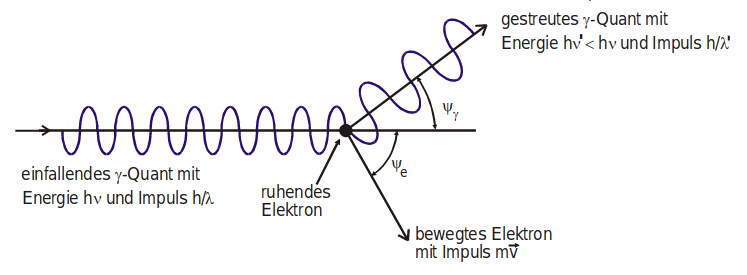
\includegraphics[width=0.8\textwidth]{compton_skizze.png}
      \caption{Darstellung des Comptoneffekts \cite{anleitungv18}.}
      \label{fig:compton_skizze}
    \end{figure}
    Die Energie des Elektrons ergibt sich zu
    \begin{align}
      E_l &= E_\gamma \,\frac{\varepsilon(1-\symup{cos}\,\Psi_\gamma)}{1+\varepsilon(1-\symup{cos}\,\Psi_\gamma)}\\
      \varepsilon &= E_\gamma\,/\,(\symup{m}_0 \symup{c}^2),
    \end{align}
    wobei $E_\gamma$ die ursprüngliche Gammaenergie, $\Psi_\gamma$ den Winkel des gestreuten Gammaquants,
    $\symup{m_0}$ die Ruhemasse des Elektrons und c die Lichtgeschwindigkeit darstellt.
    Da das Gammaquant beim Comptoneffekt nie seine gesamte Energie deponiert, ist er ein
    eher unerwünschter Effekt bei der Gammaspektroskopie. Sein Wirkungsquerschnitt $\sigma_{\symup{Co}}$ wurden von
    Klein und Nishina hergeleitet:
    \begin{align}
      \sigma_{\symup{Co}} = \frac{3}{4}\sigma_{\symup{Th}}\left(\frac{1+\varepsilon}{\varepsilon^2}\left(\frac{2+2\varepsilon}{1+2\varepsilon}-\varepsilon^{-1}\symup{ln}(1+2\varepsilon)\right)
      + \frac{1}{2\varepsilon}\symup{ln}(1+2\varepsilon) - \frac{1+3\varepsilon}{(1+2\varepsilon)^2}\right)
    \end{align}
    Dabei steht $\sigma_{\symup{Th}}$ für den Thomsonschen Streuquerschnitt.

    Bei der Paarbildung spaltet sich das Gammaquant in ein Elektron und dessen Antiteilchen, ein Positron auf.
    Dafür benötigt das Gammaquant eine Energie, die größer ist als die zweifache Ruhemasse des Elektrons.
    Da das Gammaquant in seinem eigenen Ruhesystem ruht, braucht es einen Stoßpartner für die Paarbildung.
    Aufgrund der auftretenden Rückstoßenergie, die auf den Stoßpartner wirkt, braucht es bei dem Stoß zwischen
    Gammaquant und Elektron sogar die vierfache Ruhemasse für den Paarbildungsprozess.
    Der Wirkungsquerschnitt $\sigma_{\symup{Pa}}$ der Paarbildung ist abhängig von dem Ort der Wechselwirkung.
    Je nachdem, wo in der Hülle des Atoms die Wechselwirkung stattfindet, erfährt das Gammaquant eine unterschiedlich
    starke Abschirmung.

    Zur Darstellung der Wirkungsquerschnitte der beschriebenen Wechselwirkungen ist in Abb. \ref{fig:mu_koeff}
    die Energieabhängigkeit der verschiedenen Extinktionskoeffizienten $\mu$ für Germanium abgebildet.
    \begin{figure}
      \centering
      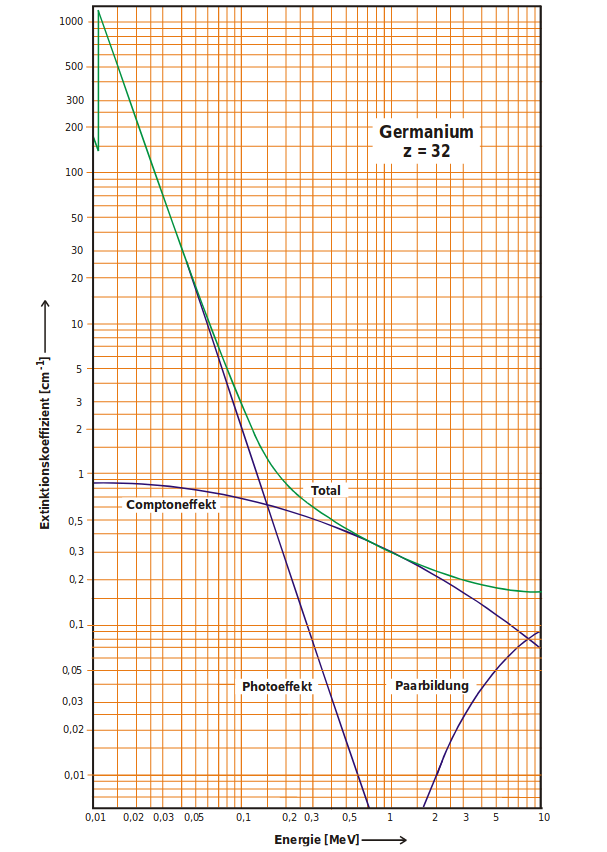
\includegraphics[width=0.95\textwidth]{mu_koeff.png}
      \caption{Extinktionskoeffizienten der verschiedenen Wechselwirkungen für Germanium \cite{anleitungv18}.}
      \label{fig:mu_koeff}
    \end{figure}

    \subsection{Funktionsweise des Reinst-Germanium-Detektors}

    Bei dem Germanium-Detektor handelt es sich um einen Halbleiter-Detektor.
    Er besteht aus einem p-dotierten- und einem n-dotierten-Bereich, welche
    sich durch einen Überschuss an Elektronen bzw. Elektronenlöchern kennzeichnen.
    An den Grenzflächen dieser Bereiche rekombinieren die Ladungsträger und bilden eine
    verarmte Zone. Diese verarmte Zone wird maximiert, indem eine äußere Spannung angelegt wird, sowie
    eine möglichst ungleich verteilte Dotierung gewählt wird. Wenn ein Gammaquant in diese
    vergrößerte verarmte Zone eindringt, enstehen mehrere
    Paare aus Elektronen und Löchern, welche durch die äußere Spannung an verschiedene
    Elektroden gesaugt werden. Dabei muss die Spannung hoch genug sein, um die Ladungsträger zu trennen,
    bevor sie rekombinieren können. Aus dem enstehenden Ladungsimpuls bei der Trennung lässt sich
    über geeignete Verfahren auf die deponierte Energie der Gammaquanten schließen.
    Die äußere Spannung darf dabei nicht zu hoch gewählt werden, da durch
    thermische Aktivierung stets ein paar Elektron-Loch-Paare enstehen, die durch die angelegte
    Spannung getrennt und als Ladungsimpulse detektiert werden. Um diesem Effekt entgegenzuwirken, wird der
    Detektor auf $\SI{77}{\kelvin}$ gekühlt.

    Der Reinst-Germanium-Detektor ist zylinderartig aufgebaut und hat den in Abb. \ref{fig:detektor}
    dargestellten Querschnitt. Seinen n-dotierten Bereich bildet die mit Lithium diffundierte Oberfläche,
    während seine innere Oberfläche mit Gold diffundiert ist und den p-dotierten Bereich darstellt.
    Um den Detektor herum ist zum Schutz eine Aluminiumschicht, welche dazu führt dass Gammaquanten erst ab einer
    bestimmten Energie detektiert werden können.
    Die gesamte Apparatur ist mit Blei umgeben, um Strahlung von außerhalb abzuhalten.
    Der Detektor kann eine Gammaenergie von einigen MeV messen.
    \begin{figure}
      \centering
      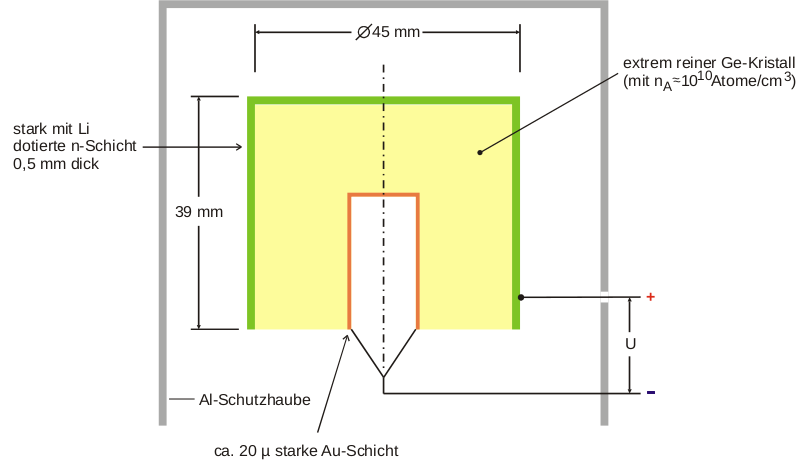
\includegraphics[width=0.95\textwidth]{detektor.png}
      \caption{Querschnitt des Reinst-Germanium-Detektor \cite{anleitungv18}.}
      \label{fig:detektor}
    \end{figure}

    Als nächstes wird auf das energetische Auflösungsvermögen des Detektors eingegangen.
    Dieses ist ein Maß dafür, wie genau der Detektor nah aneinander liegende Spektrallinien
    voneinander unterscheiden kann. Dafür wird eine Halbwertsbreite $\Delta E_{1/2}$ eingeführt, die den benötigten Abstand
    der Mittelwerte $E_1$ und $E_2$ voneinander darstellt, um eine sichere Trennung der Sprektrallinien zu gewährleisten.
    Für die Bestimmung von $\Delta E_{1/2}$ ist die Anzahl $n$ der erzeugten Elektron-Loch-Paare bei der Absorption eines
    Gammaquants entscheidend. Aus dem Verhältnis von Gammaenergie zu Bindungsenergie der Elektron-Loch-Paare, lässt sich
    der Mittelwert $\bar{n}$ bestimmen. Da jedoch das Gamma seine Energie auch zur Erzeugung von Phononen verteilt, ergibt sich
    ein Zusammenhang zwischen der Anzahl von Elektron-Loch-Paaren und den Phononen. Dies führt dazu dass der Fehler nicht mehr aus der Wurzel des
    Mittelwertes ensteht, sondern mit einem sogenannten Fano-Faktor ergänzt wird:
    \begin{align}
      \sigma = \sqrt{\symup{F}\bar{n}}
    \end{align}
    Aufgrund der vielen Elektron-Loch-Paare lässt sich die Poisson-Verteilung als
    Normalverteilung annähern, wobei gerade $\Delta E_{1/2}$ der Halbwertsbreite entspricht.
    Mit einem Fano-Faktor von 0.1 bei Germanium, ergibt sich:
    \begin{align}
      \Delta E_{1/2} = 2\sqrt{2\symup{ln}2}\,\frac{E_{\gamma}\sigma}{\bar{n}} \approx 2.35\cdot(0.1\,E_\gamma\,E_{\symup{El}})^{\frac{1}{2}}
      \label{eqn:auflsg}
    \end{align}
    Dabei steht $E_{\symup{El}}$ für die Bildungsenergie eines Paares von Elektron und Loch.
    Für einen Germanium-Detektor liegt die typische Halbwertsbreite für $\SI{500}{\kilo\electronvolt}$ bei
    $\Delta E_{1/2} =\SI{895}{\electronvolt}$.
    Problematisch für das energetische Auflösungsvermögen sind jedoch Effekte wie das Rauschen
    des Verstärkers, die Feldinhomogenität sowie der zuvor genannte
    Strom durch die thermische Aktivierung.
    Dafür wird nicht nur der Detektor, sondern auch der
    angeschlossene Verstärker gekühlt. Da die Feldinhomogenität durch eine hohe
    äußere Spannung verringert werden kann (welche den störenden Strom erhöht), muss ein Mittelmaß
    für diese gefunden werden.

    Zuletzt wird noch auf die Effizienz des Detektors eingegangen.
    Diese steht für die Energieabhängigkeit der Wahrscheinlichkeit für die vollständige Absorption
    eines Gammaquants, da nicht alle Gammaquanten ihre Energie komplett im Detektor deponieren.
    Dies folgt daraus, dass zu einer vollständige Deponierung nur der Photoeffekt fähig ist.

\section{Durchführung}
\label{sec:Durchführung}

    Zunächst wird die Schaltung des Versuches erläutert. Anschließend wird auf das
    Spektrum eines Gamma-Stahlers, welches mit dem Detektor gemessen wurde, eingegangen.

    \subsection{Elektronische Schaltung}

    Wie bereits im vorherigen Kapitel beschrieben, erzeugt der Detektor elektrische
    Ladungsimpulse, die proportional zur deponierten Gammaenergie sind. Diese Impulse werden durch
    elektrische Integration von einem kapazitiv rückgekoppelten Operationsverstärker
    in Spannungsimpulse umgewandelt. Für die Trennung der einzelnen Spannungsimpulse wird
    der eingebaute Integrationskondensator nach jedem Impuls mittels einer optoelektronischen
    Rückkopplung entladen. Diese Konstruktion bildet den sogenannten Vorverstärker.

    An den Vorverstärker angeschlossen folgt der Hauptverstärker.
    Dieser verstärkt die Spannungsimpulse auf eine Skala von 0 bis 10 Volt, und
    gibt sie anschließend an einen Analog-to-Digital-Converter (ADC) weiter.
    Dieser verwandelt die Impulse in einen brauchbaren Datensatz. Um sogenannte Pile-Ups, das
    heißt die Verwechslung von einem hohen und mehreren schnell aufeinanderfolgenden Impulsen,
    zu verhindern, wird für jeden Impuls der ADC für die benötigte Umwandlungszeit gesperrt. Dadurch
    ensteht eine effektive Totzeit, die von der gesamten gemessenen Zeit abgezogen werden muss.

    Die Impulse gelangen anschließend über einen Adressregister in einen Speicher, wo
    sie der Höhe und Anzahl nach sortiert werden, und auf den verschiedenen Kanälen
    gespeichert werden. An einem Computer lassen sich dann nach der Messzeit die gemessenen
    Signale als Impulshöhenspektrum darstellen.

    Die beschriebene Schaltung ist als Blockschaltbild in Abb. \ref{fig:blockschaltbild}
    dargestellt. Es ist dabei wichtig, den Detektor und Vorverstärker konstant auf $\SI{77}{\kelvin}$
    zu kühlen.

    \begin{figure}
      \centering
      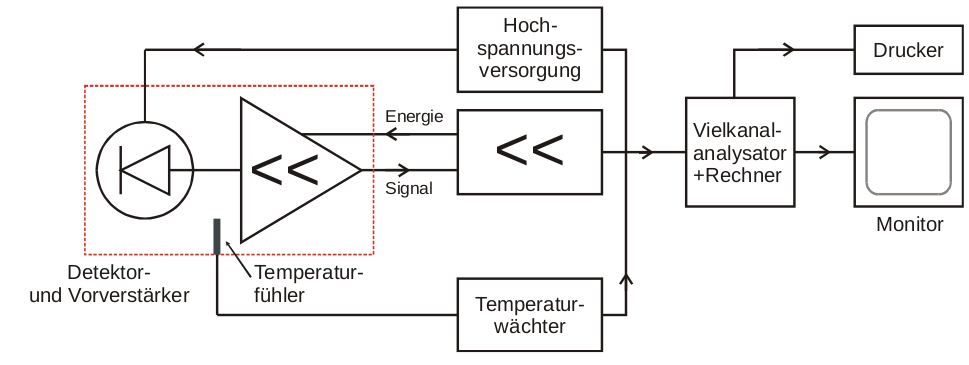
\includegraphics[width=0.95\textwidth]{blockschaltung.png}
      \caption{Blockschaltbild der elektrischen Schaltung. Der Temperaturwächter verhindert, dass die Hochspannung
      an einen Detektor angelegt wird, der nicht ausreichend gekühlt ist \cite{anleitungv18}.}
      \label{fig:blockschaltbild}
    \end{figure}

    \subsection{Energiespektrum}

    Ein beispielhaftes Spektrum eines monochromatischen Gamma-Strahlers ist in Abb. \ref{fig:spektrum}
    dargestellt. Von besonderem Interesse ist dabei der Photo- bzw. Vollenergiepeak, da
    dieser die Gammaquanten beschreibt, die ihre gesamte Energie im Detektor deponieren.
    Seine Halbwertsbreite ist die im vorherigen Kapitel beschriebene energetische Halbwertsbreite
    $\Delta E_{1/2}$ und gibt daher Auskunft über die Auflösung des Detektors.
    Das in Abb. \ref{fig:spektrum} zu sehende Compton-Kontinuum ist dagegen ein eher
    unerwünschter Effekt, da bei diesem die Gammaquanten nur einen Teil ihrer Energie deponieren.
    Es besteht zum einen aus dem Rückstreupeak, welcher durch die Gammaquanten ensteht, die
    nicht direkt in den Detektor gelangen. Damit sind vor allem die Gammaquanten gemeint die
    aus der Probe von dem Detektor weggestrahlt werden und erst über mehrere
    Wechselwirkungen mit der Umgebung in den Detektor gelangen. Zum Anderen besteht das
    Kontinuum aus der Comptonkante. Diese bezeichnet das Ende des Kontinuums und damit den
    maximalen Energieübertrag des Comptoneffekts bei einem Streuwinkel von 180°. Der
    maximale Energieübertrag beträgt dabei
    \begin{align}
      E_{\symup{max}} = 2\varepsilon\,E_\gamma\,/\,(1+2\varepsilon).
    \end{align}
    Die geringe Intensität nach der Comptonkante ensteht durch mehrfache Comptonstreuung
    von einem Gammaquant.\\
    \begin{figure}
      \centering
      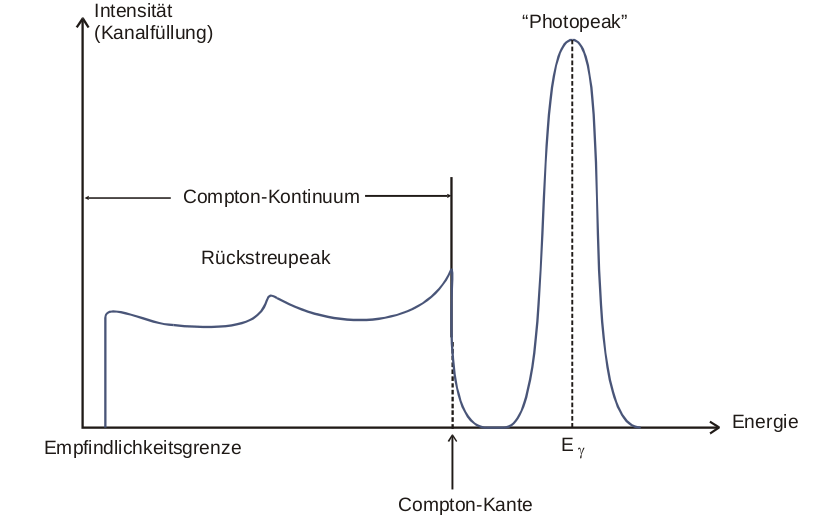
\includegraphics[width=0.95\textwidth]{spektrum.png}
      \caption{Intensität des von einem Germanium-Detektors aufgenommenen
       Energiespektrums eines monochromatischen Gamma-Strahlers  \cite{anleitungv18}.}
      \label{fig:spektrum}
    \end{figure}

    \noindent
    Um die Messergebnisse des Detektors auslesen zu können, muss eine Kalibrierung erfolgen.
    Aus dem aufgenommenen Spektrum eines bekannten Energiespektrums lässt sich mittels einer linearen
    Ausgleichsrechnung eine Umrechnungsmöglichkeit von Kanalnummer auf Energie bestimmen.
    Zusätzlich wird bei der Kalibrierung die zuvor erwähnte Effizienz Q des Detektors bestimmt, da sie
    aufgrund der vielen Linien im Spektrum dort besonders gut bestimmbar ist.
    Diese ergibt sich aus
    \begin{align}
      \symup{Q} = 4\pi\,\cdot\symup{Z}\,(\Omega\cdot\symup{A}\cdot\symup{W}\cdot t_{mess})^{-1}.
      \label{eqn:effizienz}
    \end{align}
    Dabei steht W für die Emissionswahrscheinlichkeit einer bestimmten Gammaenergie, Z für
    die Summe der Impulse in einem aufgezeichneten Peak (aus dem Spektrum ablesbar), A für die
    Aktivität des Strahlers, $\Omega$ für den Raumwinkel, unter dem der Detektor den
    Strahler sieht und $t_{mess}$ für die Messzeit. Die Aktivität A muss aus den
    Herstellerangaben für den Strahler und dem Zerfall des Nuklides bestimmt werden. Der
    Raumwinkel $\Omega$ lässt sich aus
    \begin{equation}
      \frac{\Omega}{4\pi}=\frac12\left(1-\frac a{\sqrt{a²+r²}}\right)
      \label{eqn:raum}
    \end{equation}
    berechnen, wobei der Abstand a von Probe zum Detektor groß gegenüber der Größe der Probe sein muss.
    Der Radius r des Detektors lässt sich aus Abb. \ref{fig:detektor} ablesen.

    Nach der durchgeführten Energiekalibrierung lässt sich aus aufgenommenen Energiespektren
    auf Aktivität und Nuklidart der Probe schließen.

    \subsection{Versuchsdurchführung}

    Für die Kalibrierung wird als erstes für etwa eine Stunde das bereits bekannte Energiespektrum eines
    $\ce{^{152}}\symup{Eu}$-Strahlers aufgenommen.
    Als nächstes wird circa eine Stunde lang das Spektrum eines $\ce{^{137}}\symup{Cs}$-Strahlers
    gemessen, um charakteristische Größen wie das Compton-Kontinuum oder
    den Photopeak zu erhalten.
    Anschließend wird ein Strahler für eine Stunde
    aufgezeichnet, bei dem es sich entweder um $\ce{^{125}}\symup{Sb}$ oder $\ce{^{133}}\symup{Ba}$ handelt. Es soll die Aktivität des
    Strahlers ermittelt werden.
    Zum Schluss wird zur Nuklidbestimmung ein gänzlich unbekannter Strahler gemessen.



\section{Auswertung}

  \subsection{Spektrum von Europium}

   \raggedright

    Zunächst müssen die Parameter
    $m$ und $n$ für eine Gerade der Form
    \begin{align*}
      y = m\cdot x+n
    \end{align*}
    gefunden werden. Mithilfe dieser Geraden können Kanalnummern in
    Energien umgerechnet werden.\\
    Dazu wird das Spektrum von \ce{^{152}Eu} betrachtet, weil die Energien
    der Europiumpeaks bereits bekannt sind (siehe \cite{anleitungv18}).
    In Abb. \ref{fig:euro} ist das Europium-Spektrum einmal
    normal und einmal logarithmisch zu sehen.



    \begin{figure}[H]
      \centering
      \begin{subfigure}{0.495\textwidth}
        \centering
        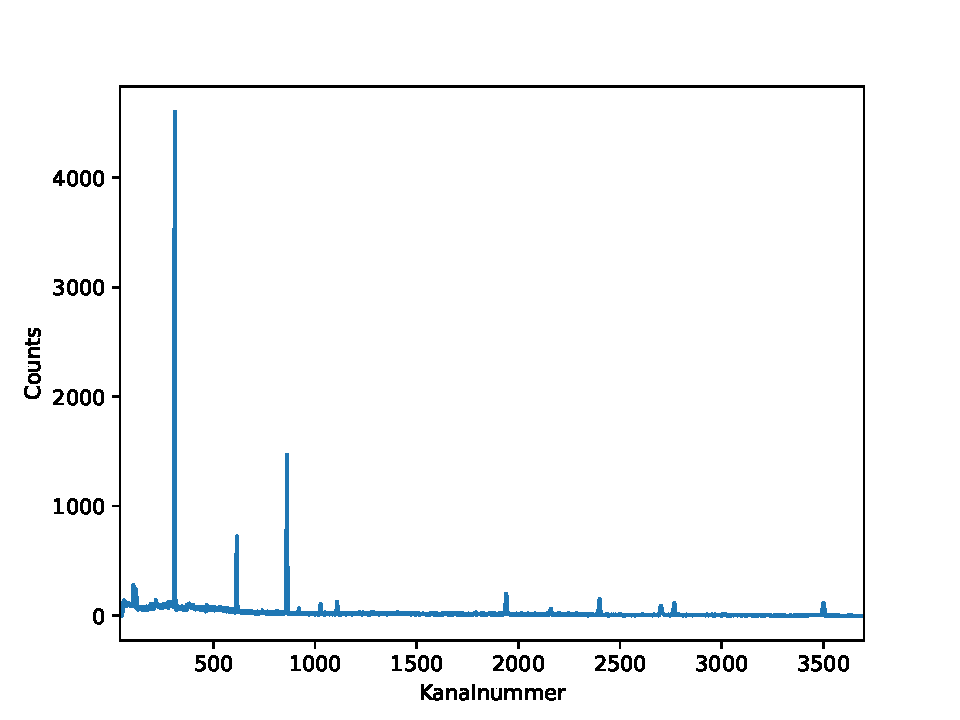
\includegraphics[height=6cm, width = 1\textwidth]{germania/eu_allgemein/europium.pdf}
      \end{subfigure}
      \begin{subfigure}{0.495\textwidth}
        \centering
        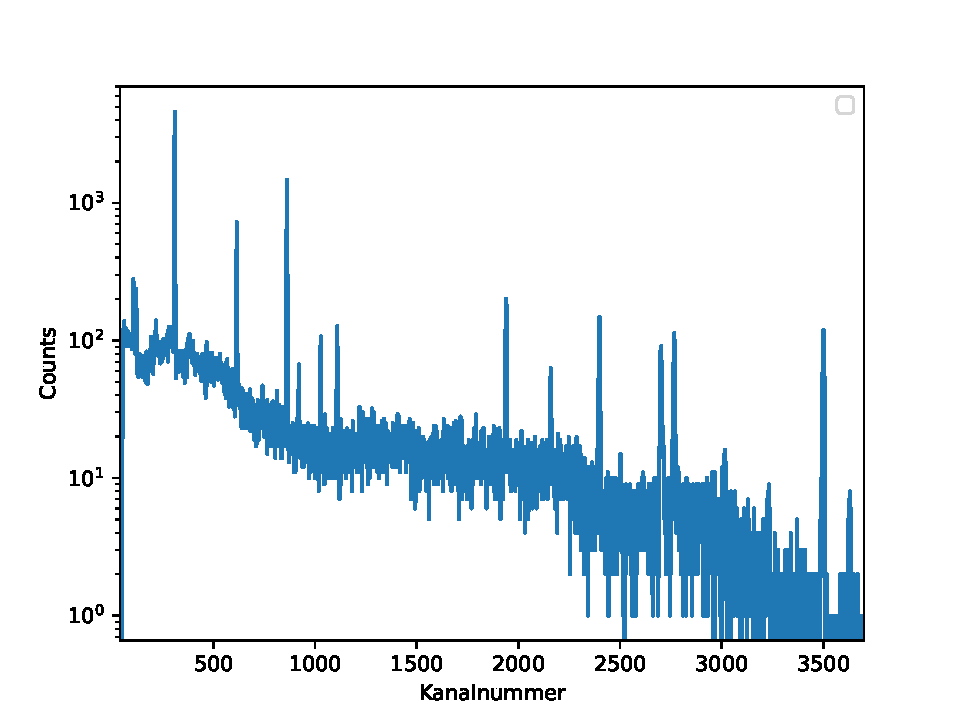
\includegraphics[height=6cm, width = 1\textwidth]{germania/eu_allgemein/europilog.pdf}
      \end{subfigure}
      \caption{Spektrum von Europium.}
      \label{fig:euro}
    \end{figure}

    Die Lage jedes Peaks wird genau bestimmt, indem er mit eine Gaußfunktion
    gefittet wird, welche die folgende Form hat:
    \begin{align*}
      G(x) = a\cdot \symup{exp}\left(-\frac12\left(\frac{x-\mu}\sigma\right)²\right).
    \end{align*}
    In Tabelle \ref{tab:kali} ist für jeden Peak die Energie angegeben sowie die Fitparameter.
    Der Parameter $\mu$ gibt dabei die Kanalnummer an, bei welcher
    die Peakenergie vorliegt, und $a$ die Anzahl der Counts im Peak.


    \begin{table}
      \centering
      \caption{Energie und Fitwerte zur Bestimmung der Peakeigenschaften.}
      \label{tab:kali}
      \begin{tabular}{c c c c c}
        \toprule
        Energie in keV & $a$ & $\mu$  & $\sigma$\\
        \midrule
        121,78 &   4650,32\pm 68,32 & 308,89\pm 0,02 &   1,18\pm 0,02\\
        244,70 &    726,64\pm 24,86 & 613,97\pm 0,06 &   1,43\pm 0,06\\
        344,30 &   1446,54\pm 14,38 & 861,02\pm 0,02 &   1,58\pm 0,02\\
        411,12 &     97,10\pm  6,70 & 1026,71\pm 0,17 &  2,19\pm 0,18\\
        443,96 &    115,79\pm  6,33 & 1108,21\pm 0,13 &  2,12\pm 0,14\\
        778,90 &    191,11\pm  9,88 & 1939,42\pm 0,16 &  2,75\pm 0,17\\
        867,37 &     55,13\pm  2,94 & 2158,75\pm 0,20 &  3,28\pm 0,21\\
        964,08 &    144,52\pm  4,03 & 2398,75\pm 0,10 &  3,12\pm 0,10\\
        1085,90 &    82,52\pm  4,45 & 2701,28\pm 0,24 &  3,80\pm 0,25\\
        1112,10 &   110,40\pm  2,92 & 2766,18\pm 0,11 &  3,60\pm 0,11\\
        1408,00 &   108,80\pm  3,83 & 3500,88\pm 0,16 &  3,97\pm 0,16\\
        \bottomrule
      \end{tabular}
    \end{table}

    Die Fits sind im Anhang in Abb. \ref{fig:fits} dargestellt.\\





    Die Mittelwerte werden nun mit den zugehörigen Energien
    in Abb. \ref{fig:regression} geplottet und
    linear gefittet. An den Mittelwerten sind Fehlerbalken.
    Da die Fehler jedoch um mehrere Größenordnungen kleiner sind als die
    Werte, sind die Fehlerbalken nicht zu erkennen.


    \begin{figure}[H]
      \centering
      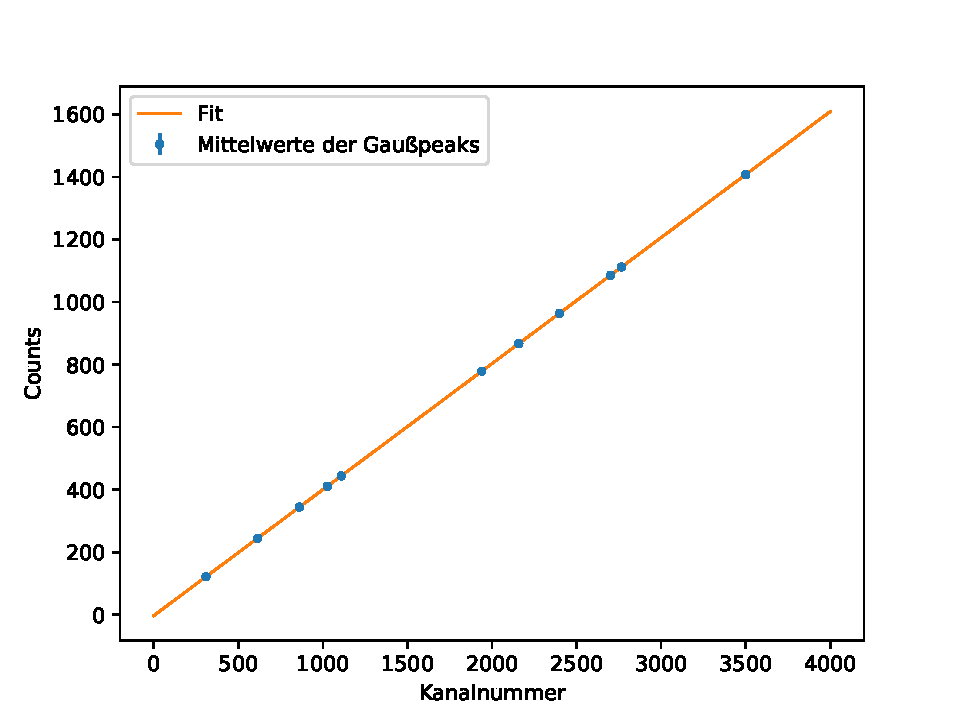
\includegraphics[height=7cm]{germania/regression/regression.pdf}
      \caption{Linearer Fit der Kanäle, deren Energien bekannt sind.}
      \label{fig:regression}
    \end{figure}

    Die Fit-Gerade hat die Parameter
    \begin{align*}
      m &= 0,40298\pm 0,00002 \,\frac{\symup{keV}}{\symup{Kanalnummer}}\\
      n &= -2,65400\pm 0,04789 \,\symup{keV}.
    \end{align*}

    Als nächstes wird der Winkel $\frac{\Omega}{4\pi}$ aus der Gleichung
    \eqref{eqn:raum}
    %\begin{align*}
    %  \frac{\Omega}{4\pi}=\frac12\left(1-\frac a{\sqrt{a²+r²}}\right)
    %\end{align*}
    berechnet.
    Dabei stellt $a$ den Abstand der Quelle vom Detektor dar und $r$
    den Radius der Querschnittsfläche des Detektors.
    Mit den Werten
    \begin{align*}
      a &= 73,2\,\text{mm}\\
      r &= 22,5\,\text{mm}
    \end{align*}
    ergibt sich für den Winkel ein Wert von 0,022.\\
    Danach wird die Aktivität der Quelle am Messtag berechnet.
    Dazu kann die Formel
    \begin{align*}
      A_{Messung}= A_0\,\symup{exp}\left(-\frac{t_{aktuell}\symup{log}(2)}{\tau_{1/2}}\right)
    \end{align*}
    verwendet werden.
    Aus der Versuchsanleitung können die Halbwertszeit $\tau_{1/2}=4943\pm 5\,\symup{d}$
    und die Aktivität $A_0=4130\pm 60\,\symup{Bq}$ vom 1.10.2000 entnommen werden.
    Zum Versuchstag waren $t_{aktuell}=6618\,\symup{d}$ vergangen.
    Damit ergibt sich für die Aktivität zum Messzeitpunkt
    $A_{Messung}=1633\pm 24\,\symup{Bq}$.\\
    Als letztes soll die Effizienz $Q$ der Spektrallinien berechnet werden,
    was mithilfe der Formel
    \begin{align*}
      Q = Z\cdot \frac{4\pi}\Omega \cdot \frac1A\cdot\frac1W\cdot\frac1{t_{mess}}
    \end{align*}
    möglich ist.
    Die Messzeit liegt bei 3960\,s.
    Die Aktivität und der Winkel sind bereits berechnet.
    $Z$ ist ebenfalls bekannt, da es die Amplitude
    des Gauspeaks darstellt.
    In Tabelle \ref{tab:effizienz} finden sich die Energien der Peaks, ihre Wahrscheinlichkeiten
    (siehe \cite{anleitungv18}),
    und die daraus berechnete Effizienz.

    \begin{table}
      \centering
      \caption{Wahrscheinlichkeiten und Effizienz der Peaks.}
      \label{tab:effizienz}
      \begin{tabular}{c c c c}
        \toprule
        Energie in keV & Wahrscheinlichkeiten & Effizienz\\
        \midrule
        121,78 & 0,286  & 0.11430\pm 0,00240    \\
        244,70 & 0,076  & 0,06720\pm 0,00250    \\
        344,30 & 0,265  & 0,03480\pm 0,00070    \\
        411,12 & 0,022  & 0,03100\pm 0,00220    \\
        443,96 & 0,031  & 0,02630\pm 0,00150    \\
        778,90 & 0,129  & 0,01040\pm 0,00060    \\
        867,37 & 0,042  & 0,00920\pm 0,00050    \\
        964,08 & 0,146  & 0,00696\pm 0,00022    \\
        1085,90 & 0,102 & 0,00569\pm 0,00032    \\
        1112,10 & 0,136 & 0,00571\pm 0,00017    \\
        1408,00 & 0,210 & 0,00364\pm 0,00014    \\
        \bottomrule
      \end{tabular}
    \end{table}

    Ein Zusammenhang zwischen der Energie und der Effizienz lässt
    sich für Energien größer 150\,keV durch eine Potenzfunktion der Form
    \begin{align*}
      Q(E)=A\cdot E^B
    \end{align*}
    finden (siehe Abb.\ref{fig:pot}).

    \begin{figure}
      \centering
      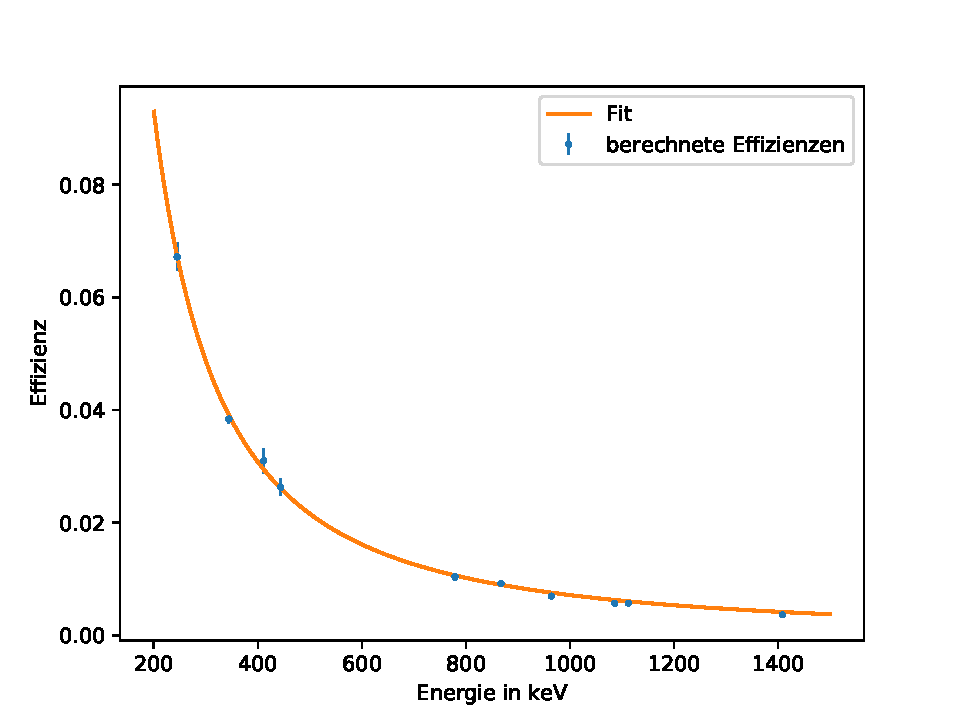
\includegraphics[height=7cm]{germania/activity/gausseffizienz.pdf}
      \caption{Fit der Effizienzen mithilfe einer Potenzfunktion.}
      \label{fig:pot}
    \end{figure}

    Es ergeben sich die Fitparameter
    \begin{align*}
      A &= 436,10\pm 61,54\\
      B &= -1,60\pm 0,02.
    \end{align*}




  \subsection{Spektrum von Caesium}

    Am Element \ce{^{137}Cs} sollen verschiedene Erscheinungen, die
    typisch für Energiespektren sind, untersucht werden.\\

    In Abb. \ref{fig:cas} ist das Caesium-Spektrum einmal
    normal und einmal logarithmisch zu sehen.

    \begin{figure}[H]
      \centering
      \begin{subfigure}{0.495\textwidth}
        \centering
        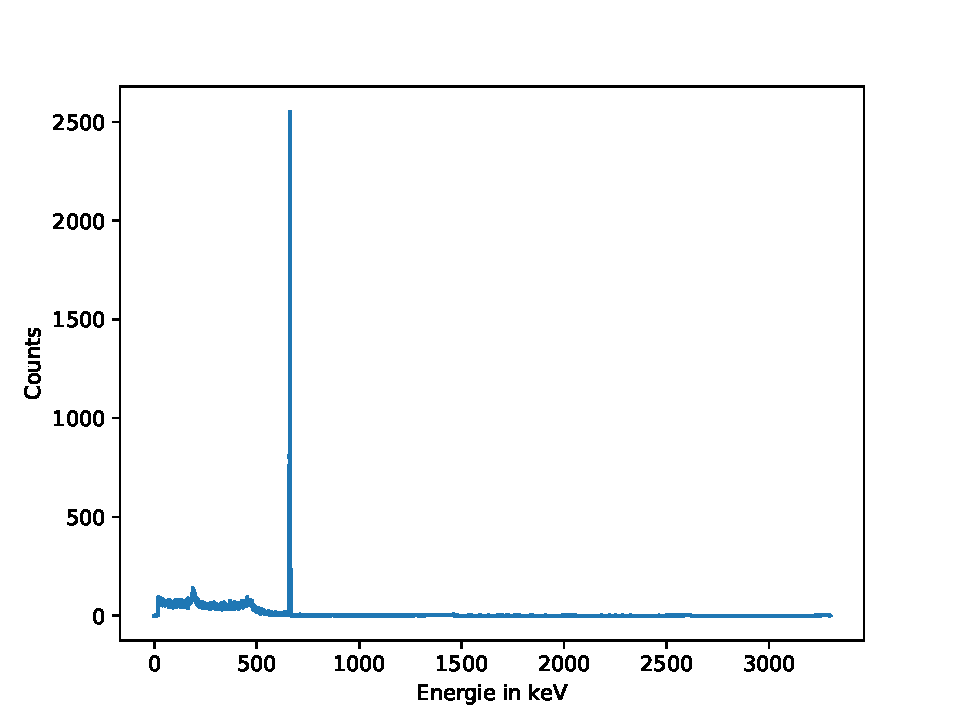
\includegraphics[height=6cm, width = 1\textwidth]{germanib/cs_allgemein/casenergie.pdf}
      \end{subfigure}
      \begin{subfigure}{0.495\textwidth}
        \centering
        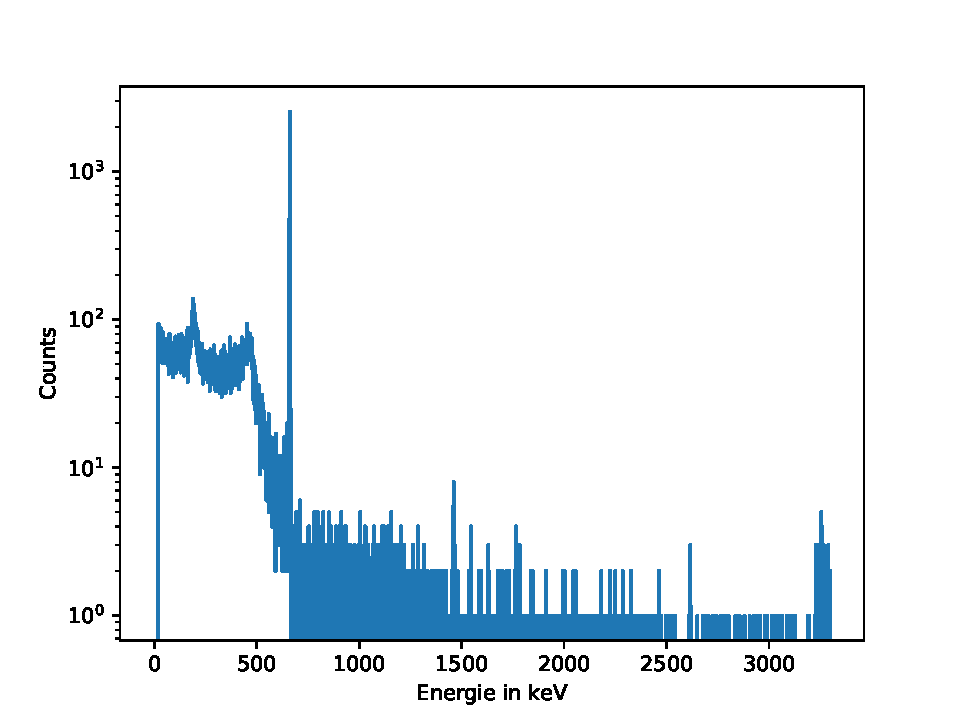
\includegraphics[height=6cm, width = 1\textwidth]{germanib/cs_allgemein/casenergielog.pdf}
      \end{subfigure}
      \caption{Spektrum von Caesium.}
      \label{fig:cas}
    \end{figure}

    Zunächst wird der Photopeak ausfindig gemacht, und wie
    im vorherigen Aufgabenteil mit einer Gaußkurve gefittet (siehe Abb.
    \ref{fig:photo}).

    \begin{figure}[H]
      \centering
      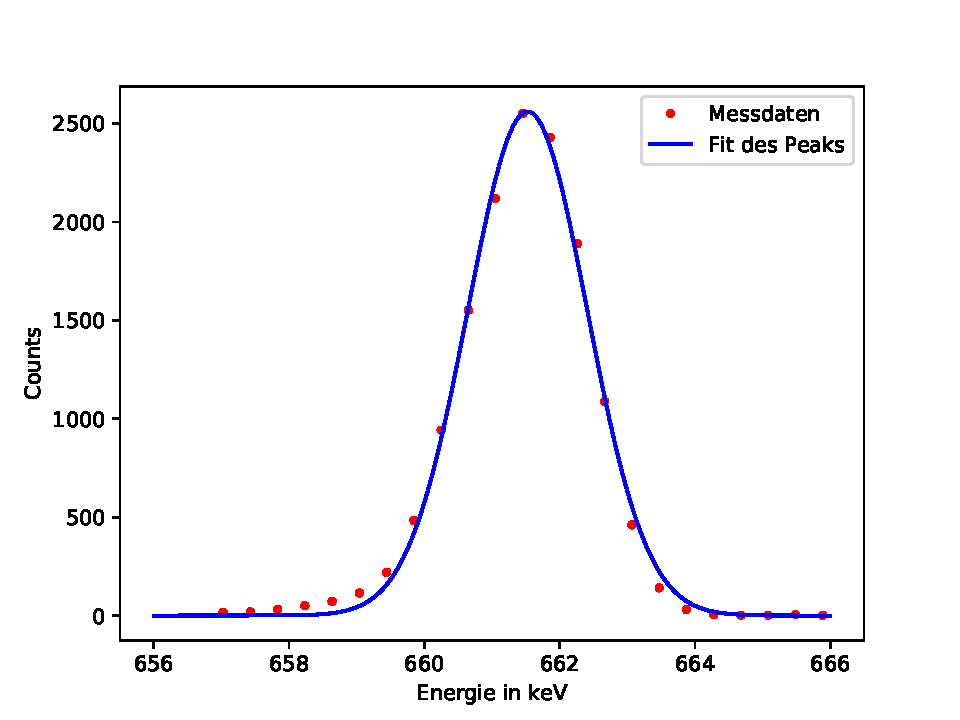
\includegraphics[height=7cm]{germanib/photo/photoenergien.pdf}
      \caption{Photopeak des Caesiumspektrums.}
      \label{fig:photo}
    \end{figure}

    Die Parameter ergeben sich zu
    \begin{align*}
      a &= 2560,73\pm 34,15\\
      \mu &= 661,52\pm 0,01\\
      \sigma &= 0,88\pm 0,01.
    \end{align*}
    Aus dem Spektrum lassen sich die Halb- und die Zehntelwertsbreite grob
    ablesen. Die Halbwertsbreite ist die Differenz von 662,46
    und 660,45\,keV, also 2,01\,keV. Die Zehntelwertsbreite ist die Differenz
    von 663,27 und 659,64\,keV, also 3,36\,keV.
    Mit diesen groben Werten liegt ein Verhältnis von
    \begin{align*}
      \frac{x_{1/10}}{x_{1/2}} = 1,81
    \end{align*}
    vor, welches nicht weit vom geforderten Verhältnis von 1,823 liegt.\\
    Ein genaueres Ergebnis lässt sich natürlich erzielen, indem die Halbwertsbreite
    aus dem durch den Fit bereits vorliegenden $\sigma$ mithilfe der Formel aus
    \cite{hwb} berechnet wird:
    \begin{align*}
      x_{1/2}=2\sqrt{2\symup{ln}(2)}\cdot\sigma = 2,077\pm 0,032\,\symup{keV}.\\
    \end{align*}
    Damit ergibt sich für die Zehntelwertsbreite:
    $x_{1/10}=x_{1/2}\cdot 1,823 = 3,79\pm 0,06.$

    Mithilfe des Photopeaks lässt sich ebenfalls die maximale Energieauflösung
    des Detektors aus der Formel \eqref{eqn:auflsg}
    %\begin{align*}
    %  \Delta E_{1/2} = 2,35\cdot \sqrt{0,1 \cdot E \cdot 2,9\,\symup{eV}}
    %\end{align*}
    berechnen. Für die Photopeakenergie ergibt sich eine Auflösung
    von $1,029\,$keV.\\

    Als nächstes wird der Rückstreupeak betrachtet.
    Die Punkte im Bereich des Rückstreupeaks sind in Abb. \ref{fig:rueck}
    geplottet. Sie sind nicht gefittet, da der Rückstreupeak keine
    Gauß-Form besitzt.

    \begin{figure}[H]
      \centering
      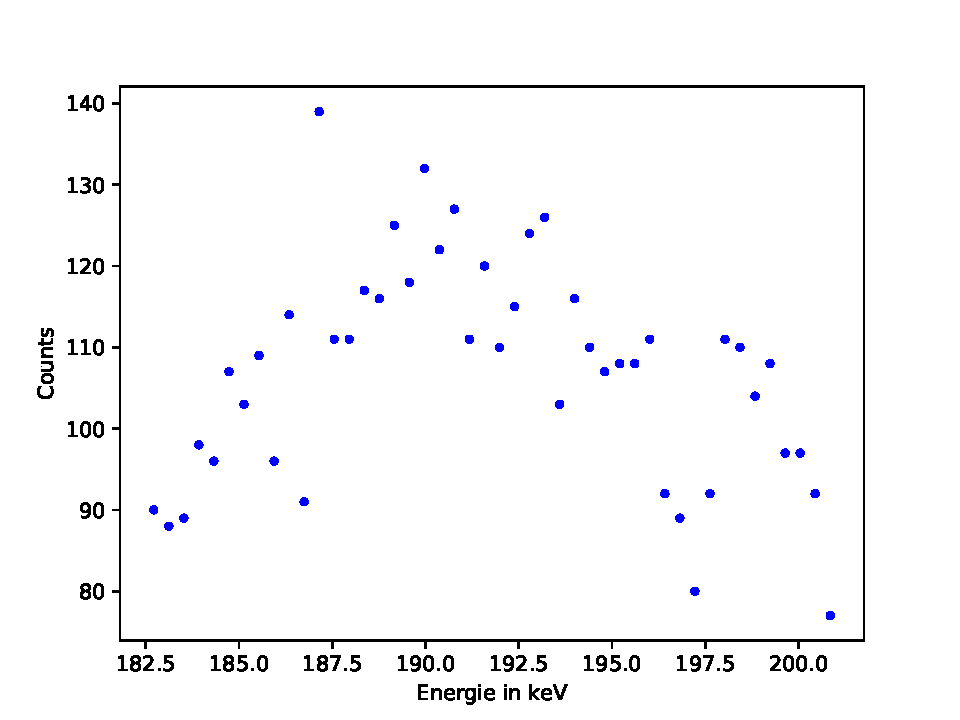
\includegraphics[height=7cm]{germanib/rueck/rueckenergie.pdf}
      \caption{Rückstreupeak des Caesiumspektrums.}
      \label{fig:rueck}
    \end{figure}

    Durch grobes Ablesen wird seine maximale Energie auf etwa 187,15\,keV
    geschätzt.
    Dies weicht von der Berechnung mithilfe der Formel
    \begin{align*}
      E_{rueck} = \frac{E_{\gamma}}{1+2\varepsilon}
    \end{align*}
    ab, da diese das Ergebnis $184,3123\pm 0,0008$ liefert. \\
    Die Comptonkante kann zunächst grob aus dem Spektrum in Abb.
    \ref{fig:comka} abgelesen werden,
    und wird bei etwa 476,49\,keV vermutet.

    \begin{figure}[H]
      \centering
      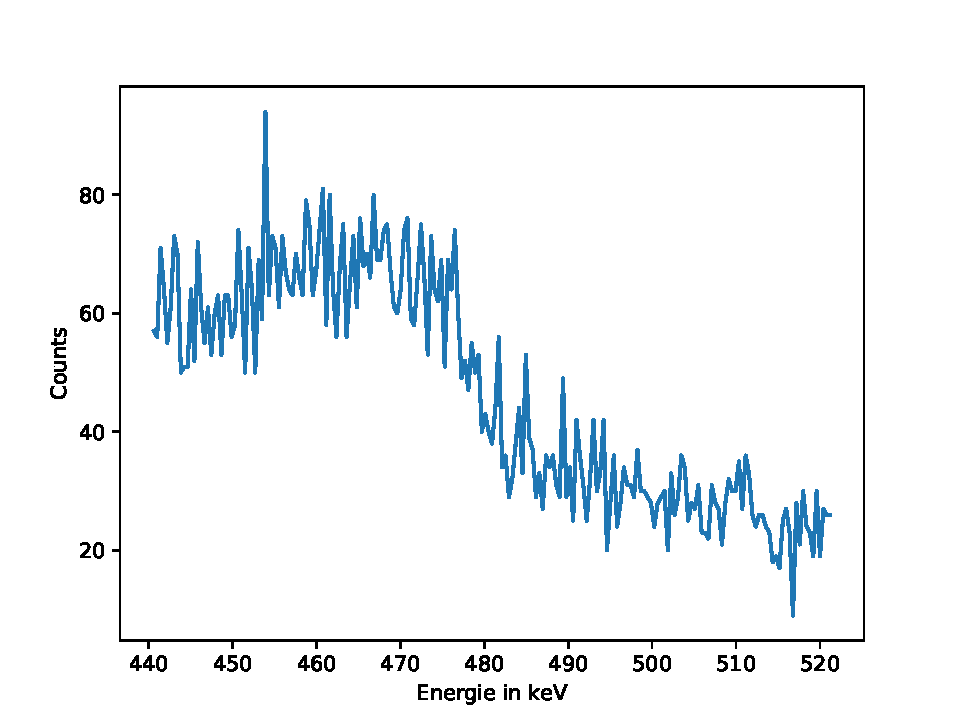
\includegraphics[height=7cm]{germanib/compton/kanteenergie.pdf}
      \caption{Comptonkante des Caesiumspektrums.}
      \label{fig:comka}
    \end{figure}


    Dies kommt dem aus
    \begin{align*}
      E_{kante}=E_{\gamma}\cdot\frac{2\varepsilon}{1+2\varepsilon}
    \end{align*}
    berechneten Wert, welcher bei $477,208\pm 0,009$ liegt, recht nahe.\\

    Das Compton-Kontinuum wird in Abb. \ref{fig:kontiganz}
    dargestellt. Um verfälschende Einflüsse niedriger Energien und
    des Rückstreupeaks zu vermeiden, wird es mit einer Funktion der Form

    \begin{align*}
      \frac{d\sigma}{dE}=
      a \cdot \sigma_{Th} \cdot \frac{1}{m_e \varepsilon²}\cdot
      \left(2+\left(\frac E{E_{\gamma}-E}\right)²\cdot \left(\frac1{\varepsilon²}+\frac{E_{\gamma}-E}{E_{\gamma}}-\frac2\varepsilon\left(\frac{E_{\gamma}-E}{E_{\gamma}}\right)\right)\right)
    \end{align*}

    approximiert, wobei für $a=10 ^{32,4}$ gilt.

    \begin{figure}[H]
      \centering
      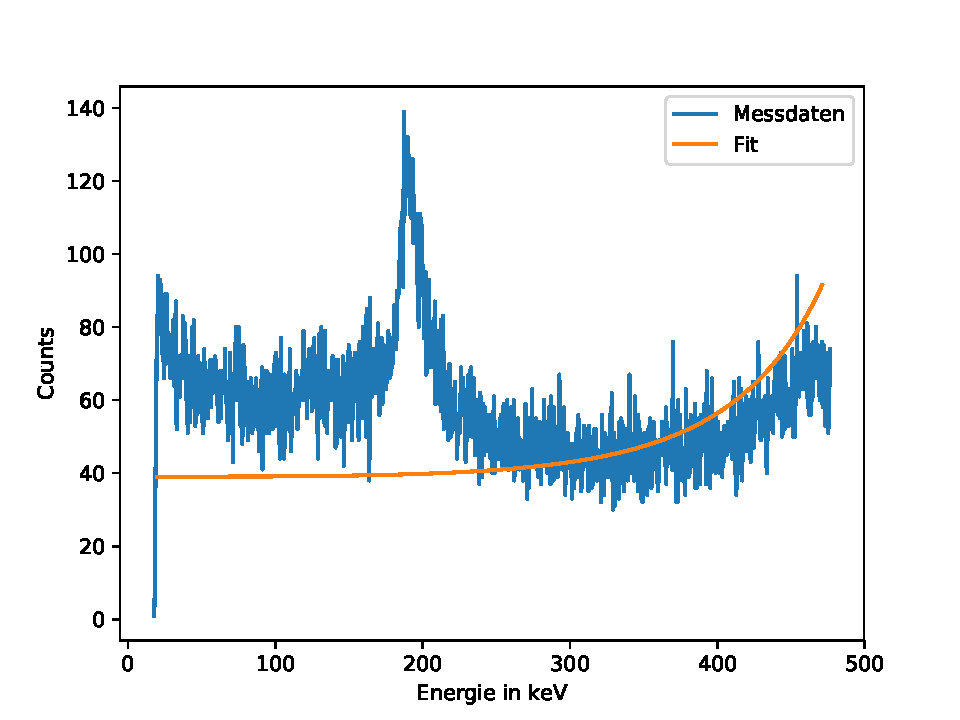
\includegraphics[height=7cm]{germanib/compton/comptonfitneu.pdf}
      \caption{Compton-Kontinuum mit Fit.}
      \label{fig:kontiganz}
    \end{figure}

    Nun wird von allen Kanälen bis zur Comptonkante der Peakinhalt unter
    der Fitfunktion berechnet und aufsummiert.
    Dadurch ergibt sich ein Compton-Kontinuumsinhalt von
    53662.93\,Counts. \\
    Das Verhältnis der Counts im Compton-Kontinuum zu denen im Photopeak
    ist
    \begin{align*}
      \frac{\text{Counts}_{compton}}{\text{Counts}_{photo}}
      \approx \frac{53662,93}{2560,73} \approx 20,96.
    \end{align*}

    Aus Abb. \ref{fig:mu_koeff} können die Absorptionskoeffizienten für den
    Compton- und den Photoeffekt bei der Energie des Photopeaks abgelesen werden:
    \begin{align*}
      \mu_{photo}& =0,008\,\frac{1}{\text{cm}}\\
      \mu_{compton}& =0,37\,\frac{1}{\text{cm}}.
    \end{align*}
    Durch Einsetzen der Absorptionskoeffizienten in
    \begin{align*}
       P_i = 1-\symup{exp}(-\mu_i\cdot d)
    \end{align*}
    ergeben sich für die Kristalllänge 3,9\,cm die Absorptionswahrscheinlichkeiten
    \begin{align*}
      P_{photo} & \approx 0,0307 = 3,07\,\% \\
      P_{compton} & \approx 0,7638 = 76,38\,\%.
    \end{align*}
    Das Verhältnis der Absorptionswahrscheinlichkeiten ist
    \begin{align*}
      \frac{P_{compton}}{P_{photo}} \approx 24,86.
    \end{align*}



  \subsection{Spektrum von Barium}

    Beim Vergleich des gemessenen Spektrums (in Abb. \ref{fig:barium}
    sowohl normal als auch logarithmisch dargestellt) mit dem Spektrum
    von \ce{^{133}Ba} wird sofort deutlich, dass es sich bei dem
    unbekannten Element um Barium handelt. \\

    \begin{figure}[H]
      \centering
      \begin{subfigure}{0.495\textwidth}
        \centering
        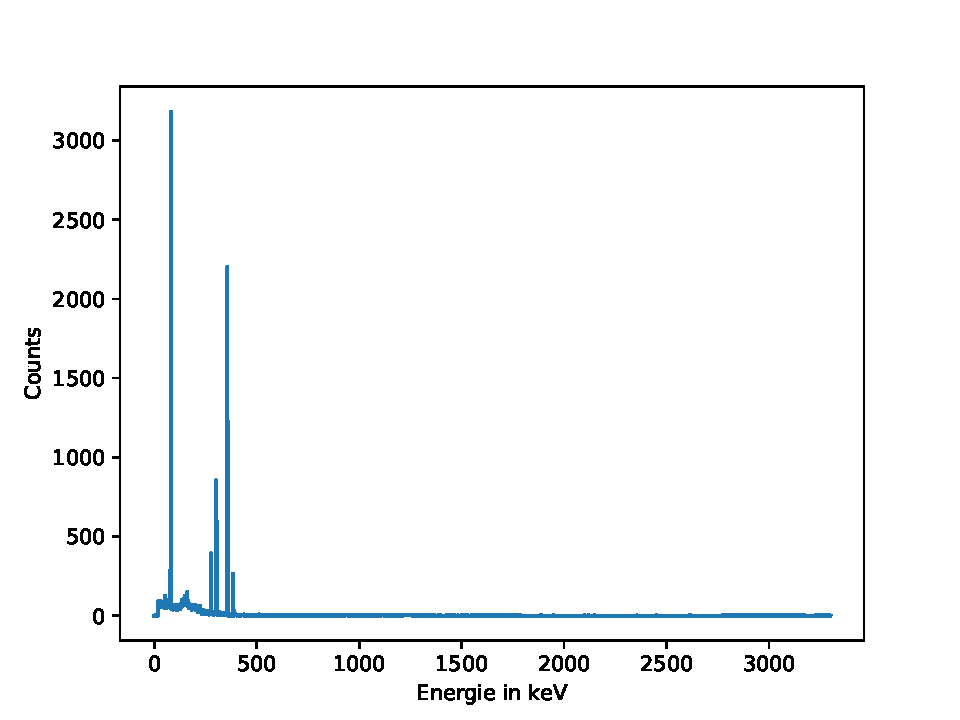
\includegraphics[height=6cm, width = 1\textwidth]{germanid/ba_allgemein/baenergie.pdf}
      \end{subfigure}
      \begin{subfigure}{0.495\textwidth}
        \centering
        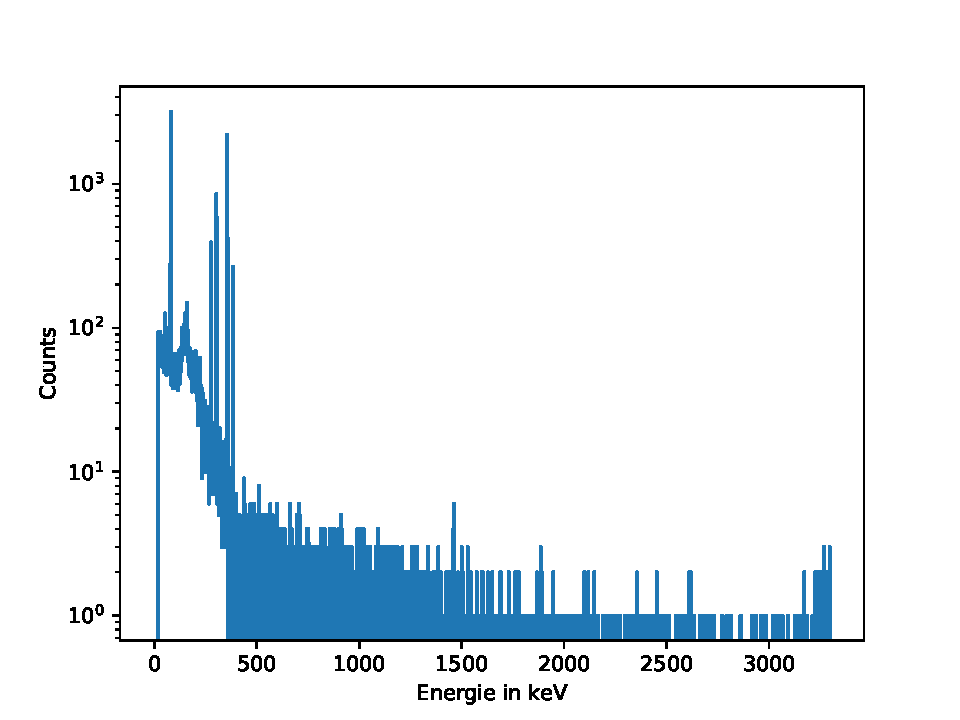
\includegraphics[height=6cm, width = 1\textwidth]{germanid/ba_allgemein/baenergielog.pdf}
      \end{subfigure}
      \caption{Spektrum von Barium.}
      \label{fig:barium}
    \end{figure}

    Sechs Barium-Peaks sind gut zu erkennen, und werden ebenfalls
    wieder mit einer Gaußkurve gefittet.
    In Tabelle \ref{tab:baren} befinden sich die charakteristischen Energien,
    und die Fitparameter $\mu$ und $a$, welche Lage und Inhalt der Peaks angeben.

    \begin{table}
      \centering
      \caption{Theoriewerte und Fit-Parameter der Barium-Peaks.}
      \label{tab:baren}
      \begin{tabular}{c c c c c}
        \toprule
        Theorieenergien & $a$ & $\mu$ \\
        \midrule
        53,16 &  113,59\pm 8,58  & 53,38\pm 0,12    \\
        81,00 &  3209,38\pm 141,82  & 81,05\pm 0,05  \\
        160,61 & 142,59\pm 4,72  & 160,68\pm 0,07  \\
        302,85 & 868,83\pm 10,15  & 302,94\pm 0,05  \\
        356,02 & 2234,23\pm 16,21  & 356,09\pm 0,05  \\
        383,85 & 278,29\pm 5,31  & 383,90\pm 0,05  \\
        \bottomrule
      \end{tabular}
    \end{table}

    Für Energien, die größer als 150\,keV sind,
    kann mithilfe der im Kapitel über Europium berechneten
    Potenzfunktion die Effizienz bestimmt werden.
    Die Messzeit beträgt 3504\,s. Übergangswahrscheinlichkeiten können
    der Quelle \cite{anleitungv18} entnommen werden.
    Damit sind für diese vier Energien sämtliche Werte
    bekannt, die zur Berechnung der Aktivität nötig sind.
    In Tabelle \ref{tab:akt} sind für diese vier Energien
    die Übergangswahrscheinlichkeiten, die berechneten Effizienzen
    und die berechneten Aktivitäten
    aufgeführt.

    \begin{table}
      \centering
      \caption{Übergangswahrscheinlichkeiten und Aktivitäten für Barium-Energien größer 150\,keV.}
      \label{tab:akt}
      \begin{tabular}{c c c c c}
          \toprule
          Energie in keV & Effizienz & Wahrscheinlichkeit & Aktivität in Bq \\
          \midrule
          160,68\pm 0,07 & 0,129\pm 0,022 & 0,006 & (2,40\pm 0,40)$\cdot 10^3$\\
          302,94\pm 0,05 & 0,047\pm 0,008 & 0,183 & (1,31\pm 0,22)$\cdot 10^3$\\
          356,09\pm 0,05 & 0,036\pm 0,007 & 0,621 & (1,30\pm 0,25)$\cdot 10^3$\\
          383,90\pm 0,05 & 0,032\pm 0,006 & 0,089 & (1,27\pm 0,24)$\cdot 10^3$\\
      \end{tabular}
    \end{table}

    Der Mittelwert der hier berechneten Aktivitäten liegt bei
    $(1,54\pm0,14)\cdot10^3\,$Bq.


  \subsection{Untersuchung einer unbekannten Quelle}

    Das Spektrum der unbekannten Quelle ist in Abb. \ref{fig:un}
    einmal normal und einmal logarithmiert zu sehen.

    \begin{figure}[H]
      \centering
      \begin{subfigure}{0.495\textwidth}
        \centering
        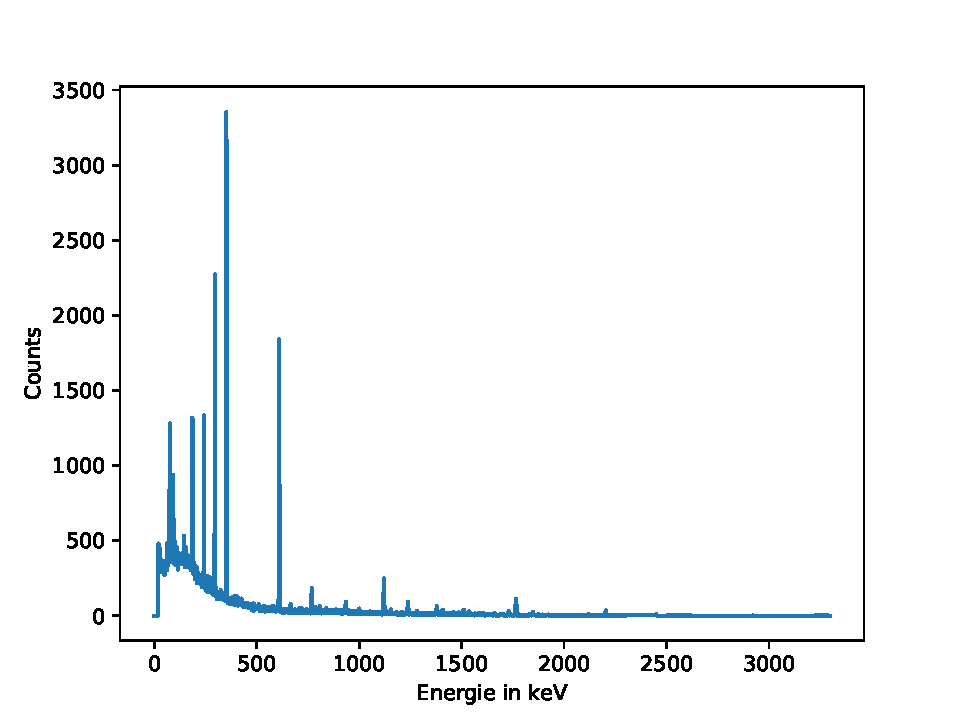
\includegraphics[height=6cm, width = 1\textwidth]{germanie/le_allgemein/leenergie.pdf}
      \end{subfigure}
      \begin{subfigure}{0.495\textwidth}
        \centering
        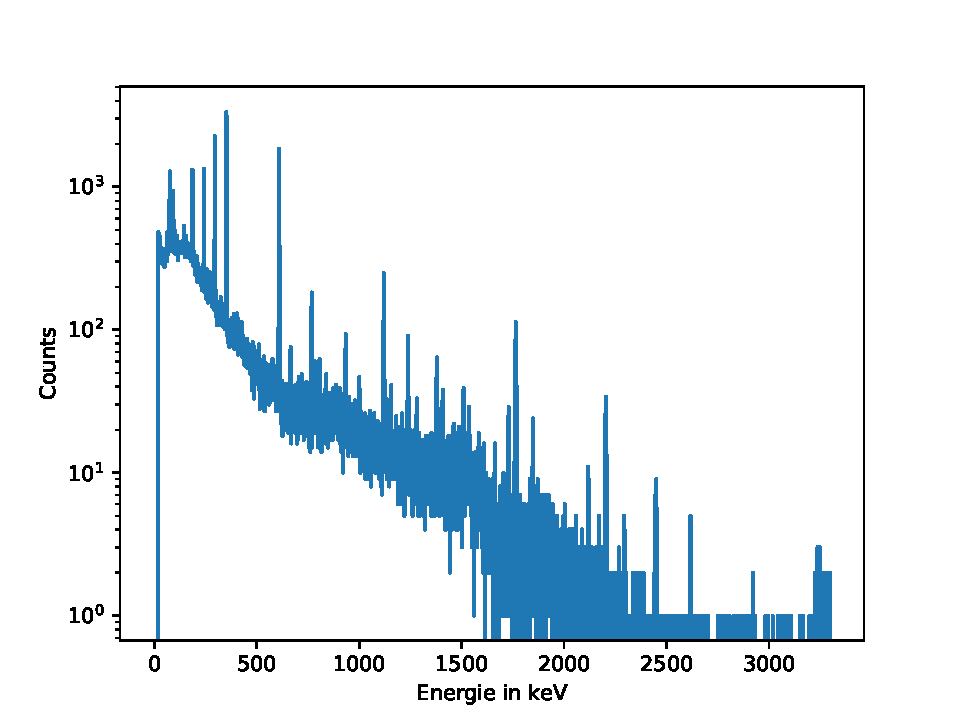
\includegraphics[height=6cm, width = 1\textwidth]{germanie/le_allgemein/leenergielog.pdf}
      \end{subfigure}
      \caption{Spektrum einer unbekannten Quelle.}
      \label{fig:un}
    \end{figure}

    Insgesamt können 23 Peaks lokalisiert werden, von welchen 21
    bekannten Elementen zuzuordnen sind.
    In Tabelle \ref{tab:gefunden} werden die Energien und Inhalte der gefundenen Peaks,
    die zugehörigen Elemente mit Theorieenergiewerten, sowie die
    Übergangswahrscheinlichkeiten angegeben.
    Die Theorieenergiewerte und Übergangswahrscheinlichkeiten sind
    den Quellen \cite{nuklide} und \cite{anleitungv18} entnommen.

    \begin{table}
        \centering
        \caption{Gefundene Peaks.}
        \label{tab:gefunden}
        \begin{tabular}{c c c c c c}
            \toprule
            Peak & $\mu$ in keV & Element & Theoriewert in keV & Wahrscheinlichkeit & $a$\\
            \midrule
            1 & 74,87\pm 0.07 & \ce{^{161} Dy} & 74,60 & 0,599      & 908,80\pm 39,46      \\
            2 & 77,10\pm 0.06 & \ce{^{161} Dy} & 77,40 & 0,560      & 1229,26\pm 53,33      \\
            3 & 87,24\pm 0.07 & \ce{^{161} Dy} & 87,90 & 0,102      & 755,64\pm 33,04      \\
            4 & 92,66\pm 0.06 & \ce{^{234} Th} & 93,00 & 0,040      & 943,68\pm 31,04      \\
            5 & 186,09\pm 0.06 & \ce{^{226} Ra} & 186,00 & 0,040    & 1343,38\pm 48,56      \\
            6 & 242,07\pm 0.06 & \ce{^{214} Pb} & 242,00 & 0,040    & 1315,49\pm 64,60     \\
            7 & 295,29\pm 0.05 & \ce{^{214} Pb} & 295,00 & 0,190    & 2320,78\pm 62,48      \\
            8 & 351,96\pm 0.05 & \ce{^{214} Pb} & 352,00 & 0,360    & 3392,74\pm 51,45      \\
            9 & 609,20\pm 0.06 & \ce{^{214} Bi} & 609,00 & 0,470    & 1873,31\pm 29,54      \\
            10 & 665,48\pm 0.11 & \ce{^{161} Dy} & 665,39 & 0,300   & 75,76\pm 4,31      \\
            11 & 768,20\pm 0.10 & \ce{^{214} Bi} & 769,00 & 0,050   & 166,39\pm 7,98      \\
            12 & 785,98\pm 0.17 & \ce{^{212} Bi} & 787,00 & 0,012   & 56,42\pm 7,55      \\
            13 & 933,86\pm 0.07 & \ce{^{214} Bi} & 935,00 & 0,030   & 93,12\pm 0,43      \\
            14 & 1000,75\pm 0.12 & \ce{^{58} Co} & 1000,70 & 1,000  & 42,00\pm 2,81      \\
            15 & 1120,30\pm 0.09 & \ce{^{214} Bi} & 1120,00 & 0,170 & 252,43\pm 8,24      \\
            16 & 1238,00\pm 0.09 & \ce{^{58} Co} & 1236,50 & 1,000  & 87,39\pm 1,85      \\
            17 & 1378,19\pm 0.13 & \ce{^{214} Bi} & 1378,00 & 0,050 & 59,25\pm 2,97      \\
            18 & 1509,60\pm 0.22 & \ce{^{214} Bi} & 1509,00 & 0,020 & 35,68\pm 3,05      \\
            19 & 1729,28\pm 0.26 & \ce{^{214} Bi} & 1728,00 & 0,030 & 25,64\pm 2,84      \\
            20 & 1764,67\pm 0.13 & \ce{^{214} Bi} & 1764,00 & 0,170 & 118,25\pm 3,64      \\
            21 & 1848,06\pm 0.14 & unbekannt & -   & -                 & 21,45\pm 1,31      \\
            22 & 2117,02\pm 0.21 & unbekannt & -   & -                 & 10,69\pm 2,38      \\
            23 & 2204,16\pm 0.14 & \ce{^{214} Bi} & 2204,00 & 0,050 & 32,42\pm 3,26     \\
            \bottomrule
        \end{tabular}
    \end{table}


    Der Tabelle ist zu entnehmen, dass der Strahler \ce{^{234}Thorium},
    \ce{^{226}Radium}, \ce{^{214}Bismuth} und \ce{^{214}Blei} aus der
    \ce{^{238}Uran}-Zerfallsreihe beinhaltet. \\
    Aus der \ce{^{232}Thorium}-Zerfallsreihe ist nur \ce{^{212}Bismuth} vertreten.\\
    Außerdem sind Spektrallinien von \ce{^{58}Cobalt} und \ce{^{161}Dysprosium}
    zu erkennen, welche keine Glieder der am häufigsten vorkommenden Zerfallsreihen sind.


\section{Diskussion}

  Die für die Kalibrierung errechneten Mittelwerte liegen sehr genau auf einer
  Geraden, weshalb die Parameter $m$ und $n$ nur geringe Fehler besitzen.
  Daher führt die Kalibrierung in weiteren Aufgabenteilen nur zu geringen
  Fehlern. \\
  Die Potenzfunktion, welche einen Zusammenhang zwischen Energie und Effizienz
  darstellt, ist ebenfalls eine gute Approximation, da die meisten
  Effizienzen auf ihr liegen, und die abweichenden nicht weit von ihr entfernt sind.\\
  Der Wert des Vollenergiepeaks weicht um 0,52\,keV vom Literaturwert ab.
  \cite{nuklide}
  Dies ist auf kleine Ungenauigkeiten beim Fitten und bei der Regressionsrechnung
  zurückzuführen.\\
  Der abgelesene Rückstreupeak liegt deutlich vom berechneten entfernt.
  Die Ursache liegt in Ableseungenauigkeiten.\\
  Die Comptonkante ist für das Auge besser zu erkennen, weshalb
  dort die Abweichung zwischen abgelesenem und errechnetem Wert
  vernachlässigbar gering ist.\\
  Das gemessene Verhältnis von Comptoneffekt zu Photoeffekt ist kleiner
  als das berechnete, was Sinn ergibt, da in der Anleitung bereits angedeutet
  wird, dass der mit der verwendeten Formel errechnete Wert für den Photoeffekt zu niedrig ist im Vergleich
  mit experimentell ermittelten Werten.\\
  Die gemessenen und gefitteten Werte für Barium unterscheiden sich
  erst nach dem Komma von den Literaturwerten. Kleine Abweichungen
  kommen zustande, da die leicht fehlerbehaftete Kalibrierung durch Europium
  verwendet wird, und die Peaks ihrerseits gefittet werden.\\
  Die Energiewerte der unbekannten Quelle weichen teilweise etwas deutlicher,
  also in der Größenordnung von 1\,eV,
  von den Literaturwerten der vermuteten Elemente ab.
  Dies kommt zum einen durch die erhöhte Peakdichte, welche die Ermittelung und
  den Fit einzelner Peaks schwerer macht. Andererseits könnte auch hinter
  einigen Peaks das falsche Element vermutet worden sein.


\section{Anhang}


    \begin{figure}
      \centering
      \begin{subfigure}{0.31\textwidth}
        \centering
        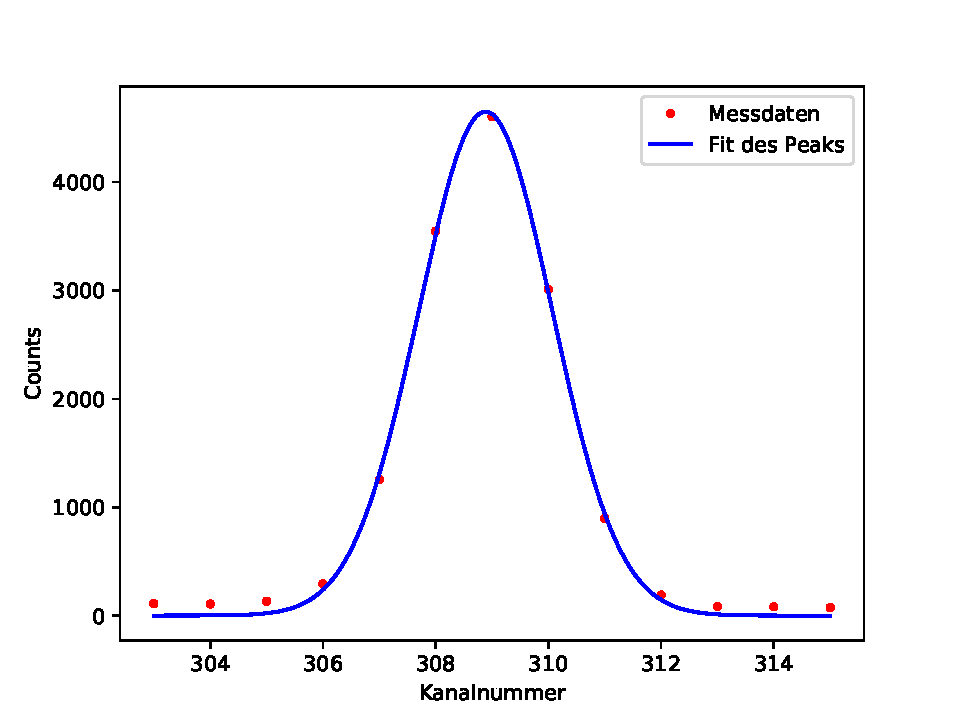
\includegraphics[height=5cm, width=1\textwidth]{germania/peak1/peak1.pdf}
        \caption{Peak zu 121,78\,keV.}
      \end{subfigure}
      \begin{subfigure}{0.31\textwidth}
        \centering
        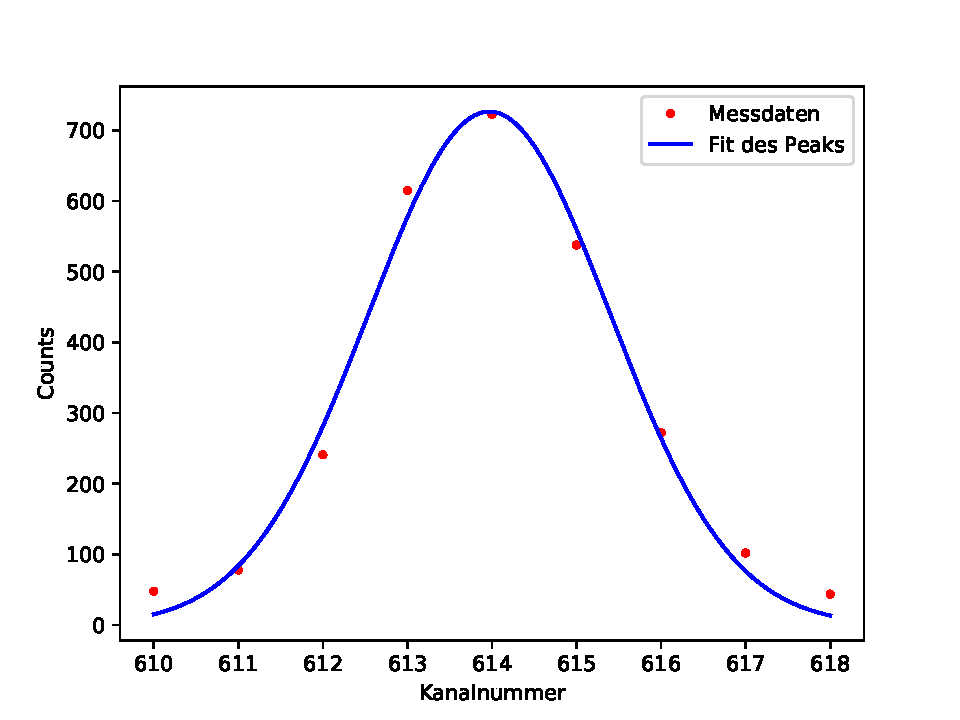
\includegraphics[height=5cm, width=1\textwidth]{germania/peak2/peak2.pdf}
        \caption{Peak zu 224,70\,keV.}
      \end{subfigure}
      \begin{subfigure}{0.31\textwidth}
        \centering
        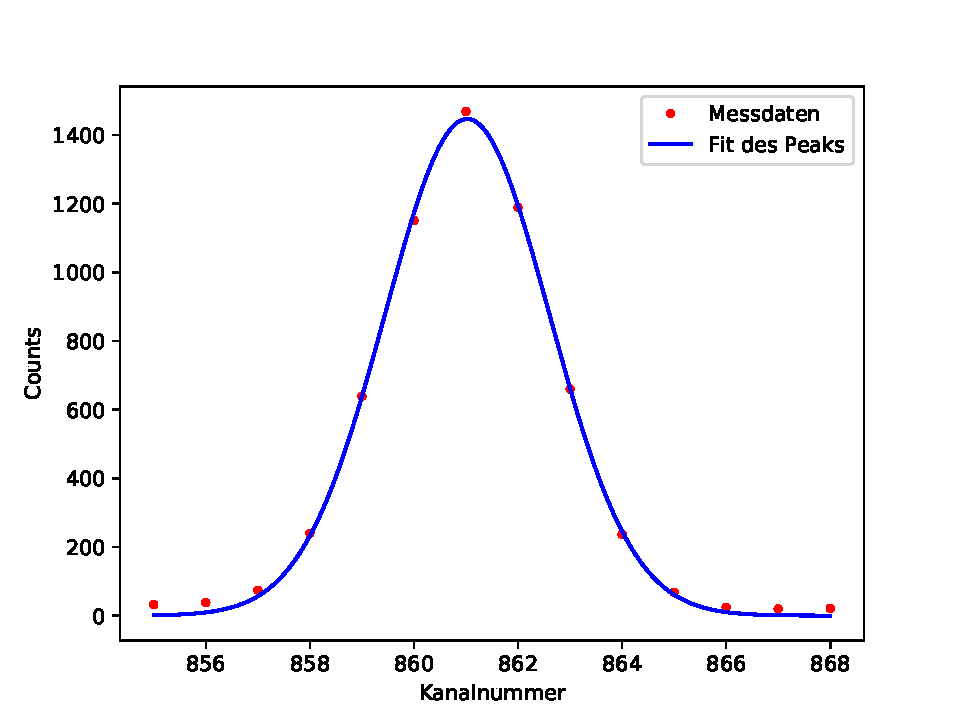
\includegraphics[height=5cm, width=1\textwidth]{germania/peak3/peak3.pdf}
        \caption{Peak zu 344,30\,keV.}
      \end{subfigure}\\
      \begin{subfigure}{0.33\textwidth}
        \centering
        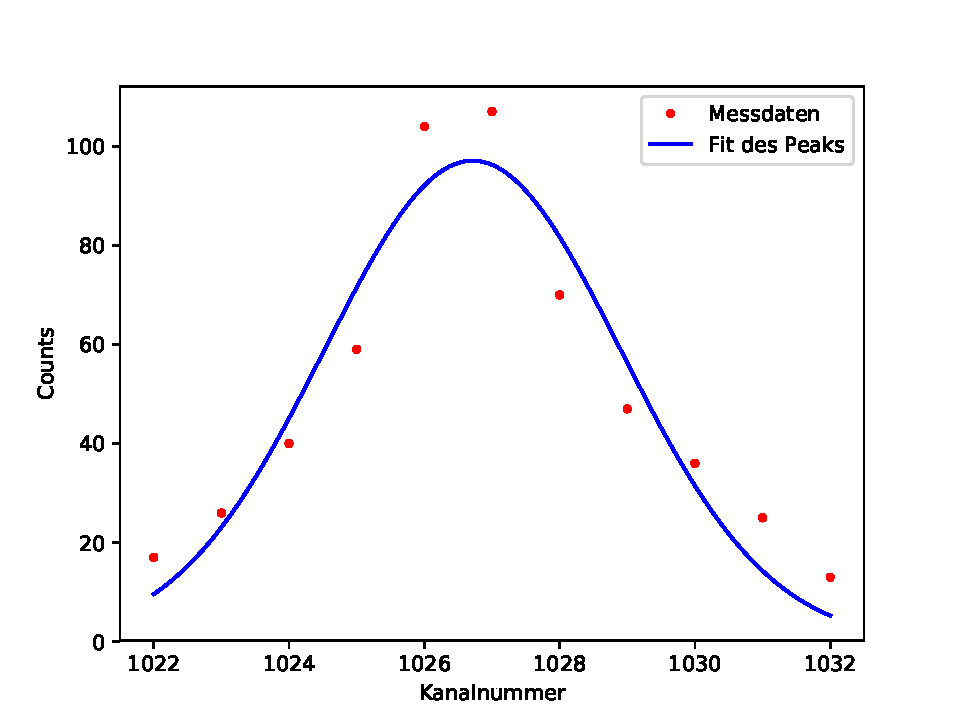
\includegraphics[height=5cm, width=1\textwidth]{germania/peak4/peak4.pdf}
        \caption{Peak zu 411,12\,keV.}
      \end{subfigure}
      \begin{subfigure}{0.31\textwidth}
        \centering
        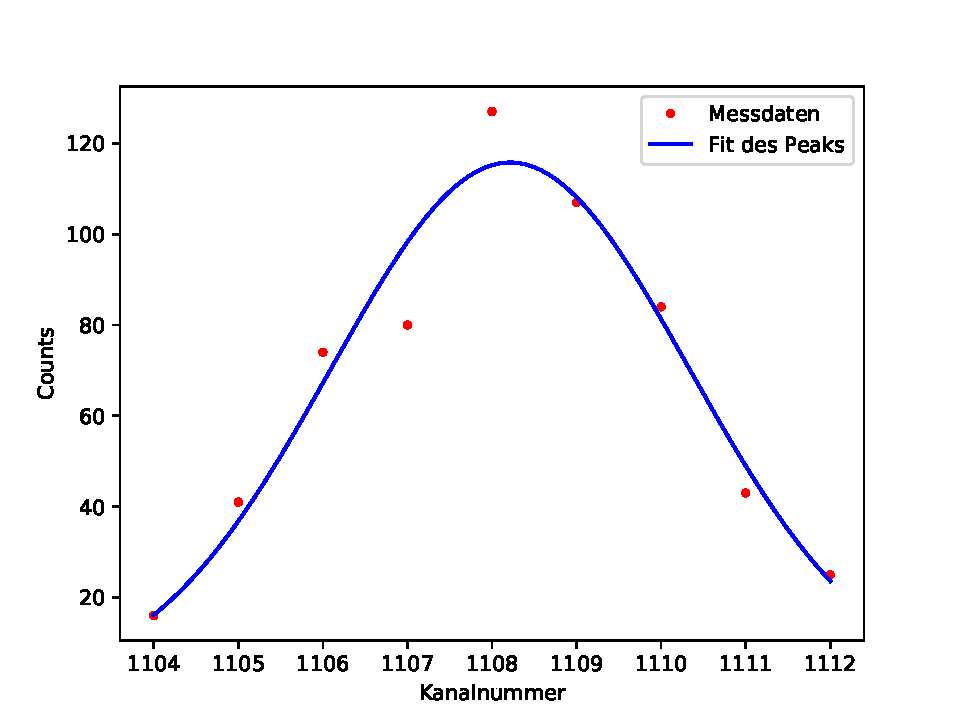
\includegraphics[height=5cm, width=1\textwidth]{germania/peak5/peak5.pdf}
        \caption{Peak zu 443,96\,keV.}
      \end{subfigure}
      \begin{subfigure}{0.31\textwidth}
        \centering
        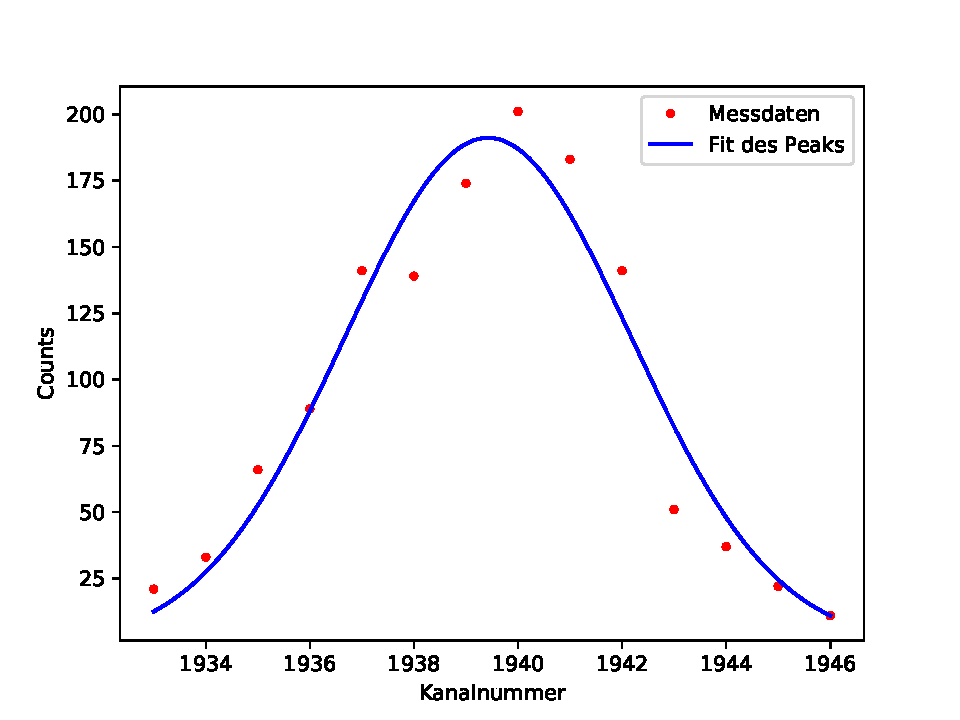
\includegraphics[height=5cm, width=1\textwidth]{germania/peak6/peak6.pdf}
        \caption{Peak zu 778,90\,keV.}
      \end{subfigure}\\
      \begin{subfigure}{0.31\textwidth}
        \centering
        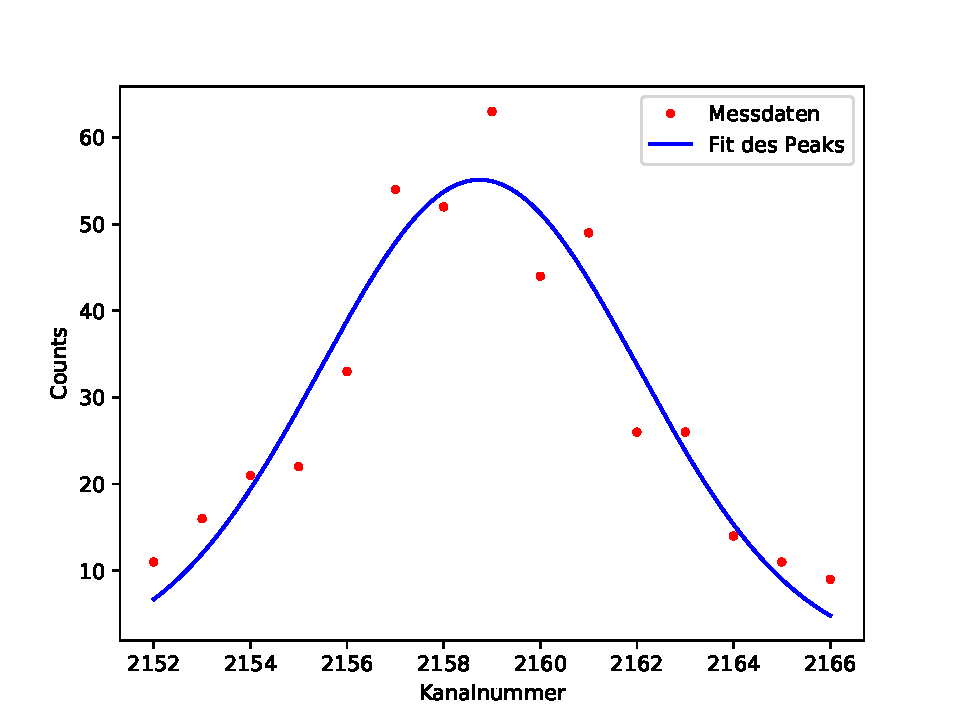
\includegraphics[height=5cm, width=1\textwidth]{germania/peak7/peak7.pdf}
        \caption{Peak zu 867,37\,keV.}
      \end{subfigure}
      \begin{subfigure}{0.31\textwidth}
        \centering
        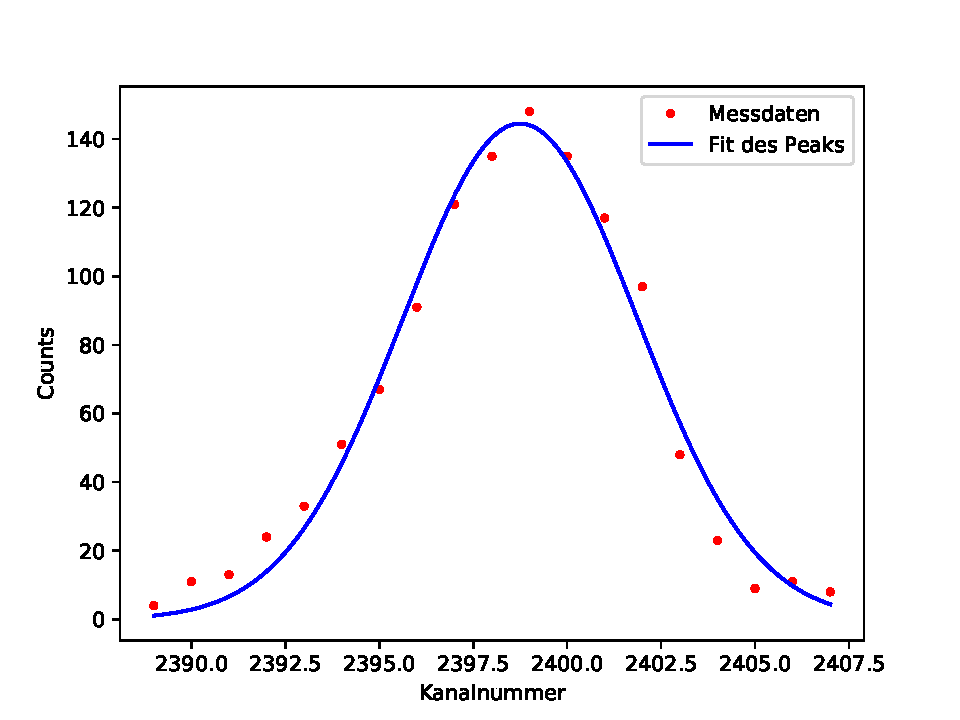
\includegraphics[height=5cm, width=1\textwidth]{germania/peak8/peak8.pdf}
        \caption{Peak zu 964,08\,keV.}
      \end{subfigure}
      \begin{subfigure}{0.31\textwidth}
        \centering
        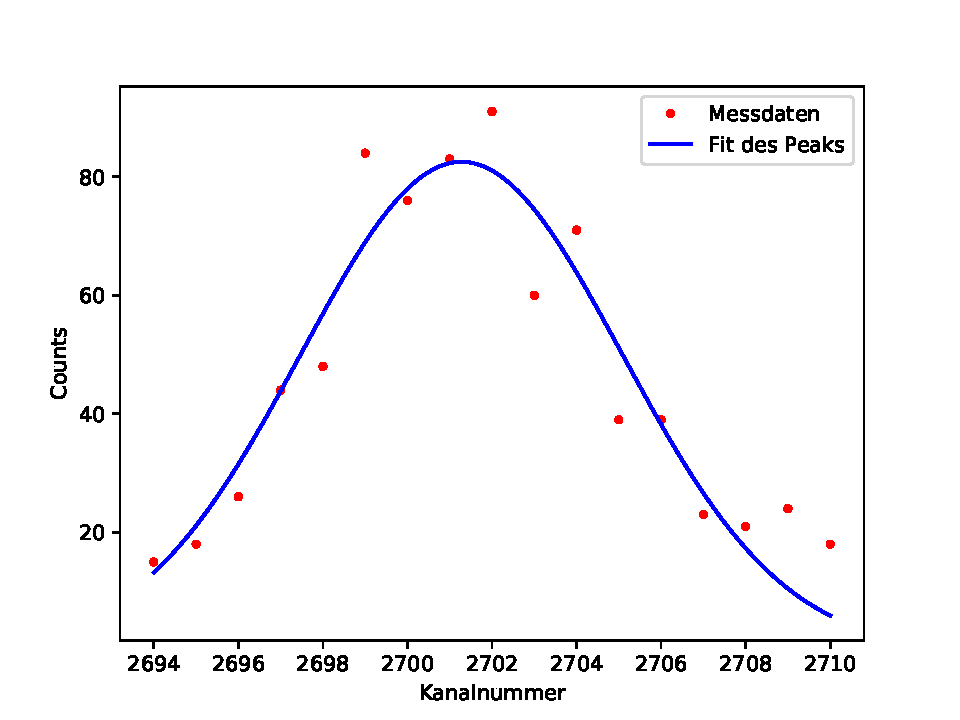
\includegraphics[height=5cm, width=1\textwidth]{germania/peak9/peak9.pdf}
        \caption{Peak zu 1085,90\,keV.}
      \end{subfigure}\\
      \begin{subfigure}{0.31\textwidth}
        \centering
        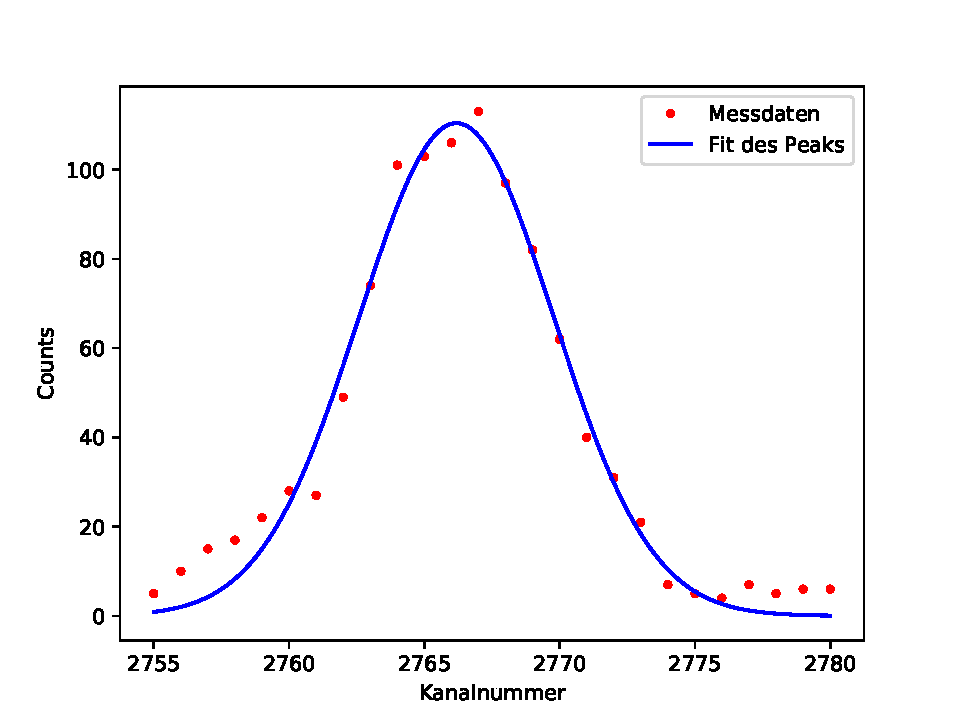
\includegraphics[height=5cm, width=1\textwidth]{germania/peak10/peak10.pdf}
        \caption{Peak zu 1112,10\,keV.}
      \end{subfigure}
      \begin{subfigure}{0.31\textwidth}
        \centering
        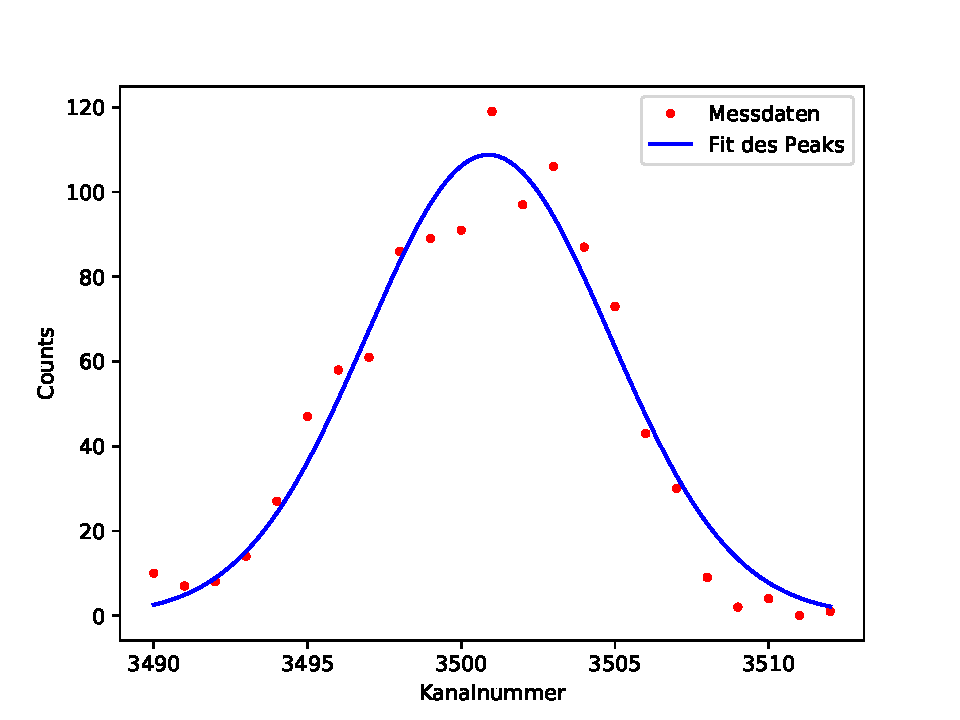
\includegraphics[height=5cm, width=1\textwidth]{germania/peak11/peak11.pdf}
        \caption{Peak zu 1408,00\,keV.}
      \end{subfigure}
      \caption{Mit Gaußkurven gefittete Peaks des Europiumspektrums.}
      \label{fig:fits}
    \end{figure}

\printbibliography

\end{document}
